% !TeX root=main.tex
%% دو سری دستور زیر باید در اولین فایل پیوست باشند. آنها را حذف نکنید!
% دستورات لازم برای تبدیل «فصل آ» به «پیوست آ» در فهرست مطالب
\addtocontents{toc}{
    \protect\renewcommand\protect\cftchappresnum{\appendixname~}%
    \protect\setlength{\cftchapnumwidth}{\mylenapp}}
    
\let\Chapter\chapter
% دستورات لازم برای شماره‌گذاری صفحات پیوست‌ها بشکل آ-۱ (فعلا با glossaries سازگار نیست)
% \pretocmd{\chapter}{
%  \clearpage
%  \pagenumbering{arabic}
%  \renewcommand*{\thepage}{\rl{\thechapter-\arabic{page}}}}{}{}
%%%%%%%%%%%%%%%%%%%%%%%%%%%%%%%%%%%%%
    
\chapter{پرسشنامه‌ها}
\label{app:questionnaires}
پرسشنامه ۱
% 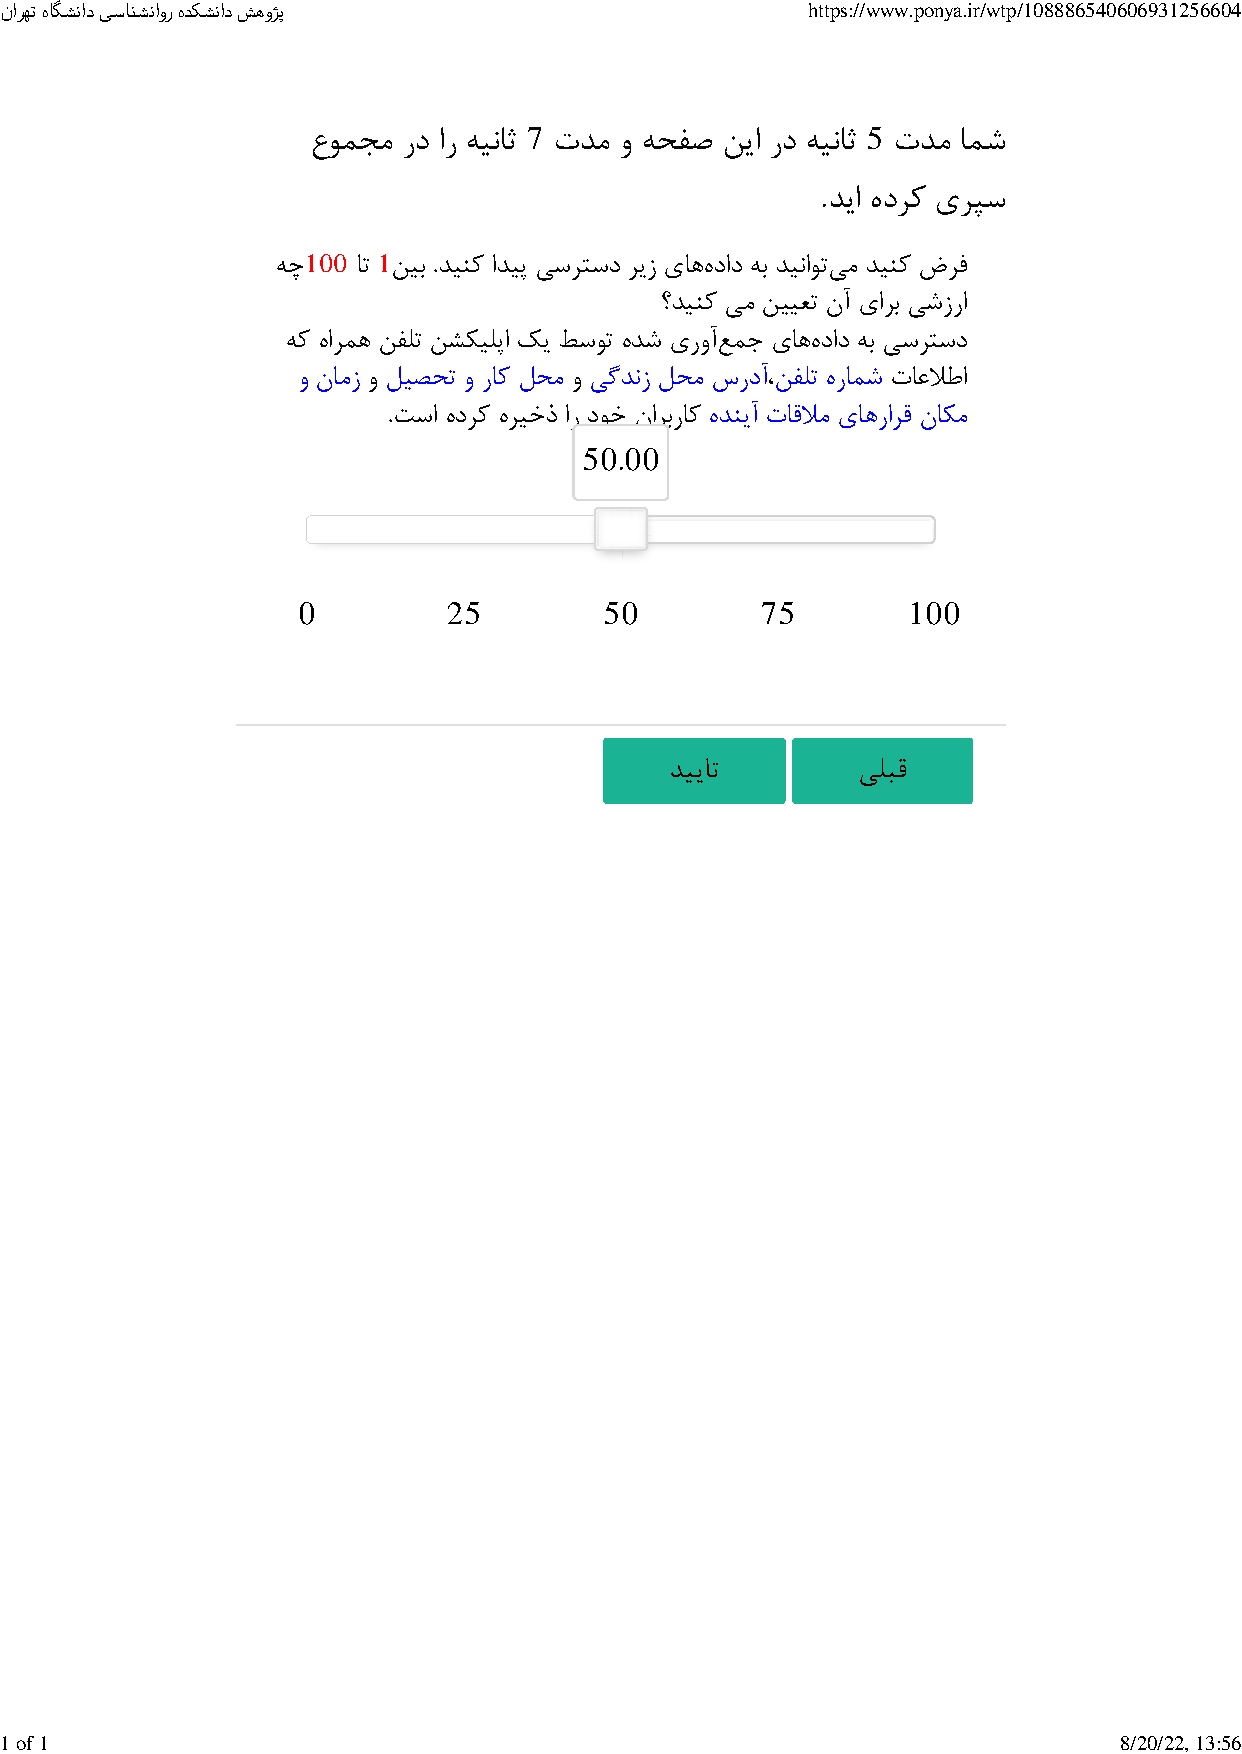
\includepdf[pages={1-3,{},8,10-12}]{questionnares/wtp.pdf}
% 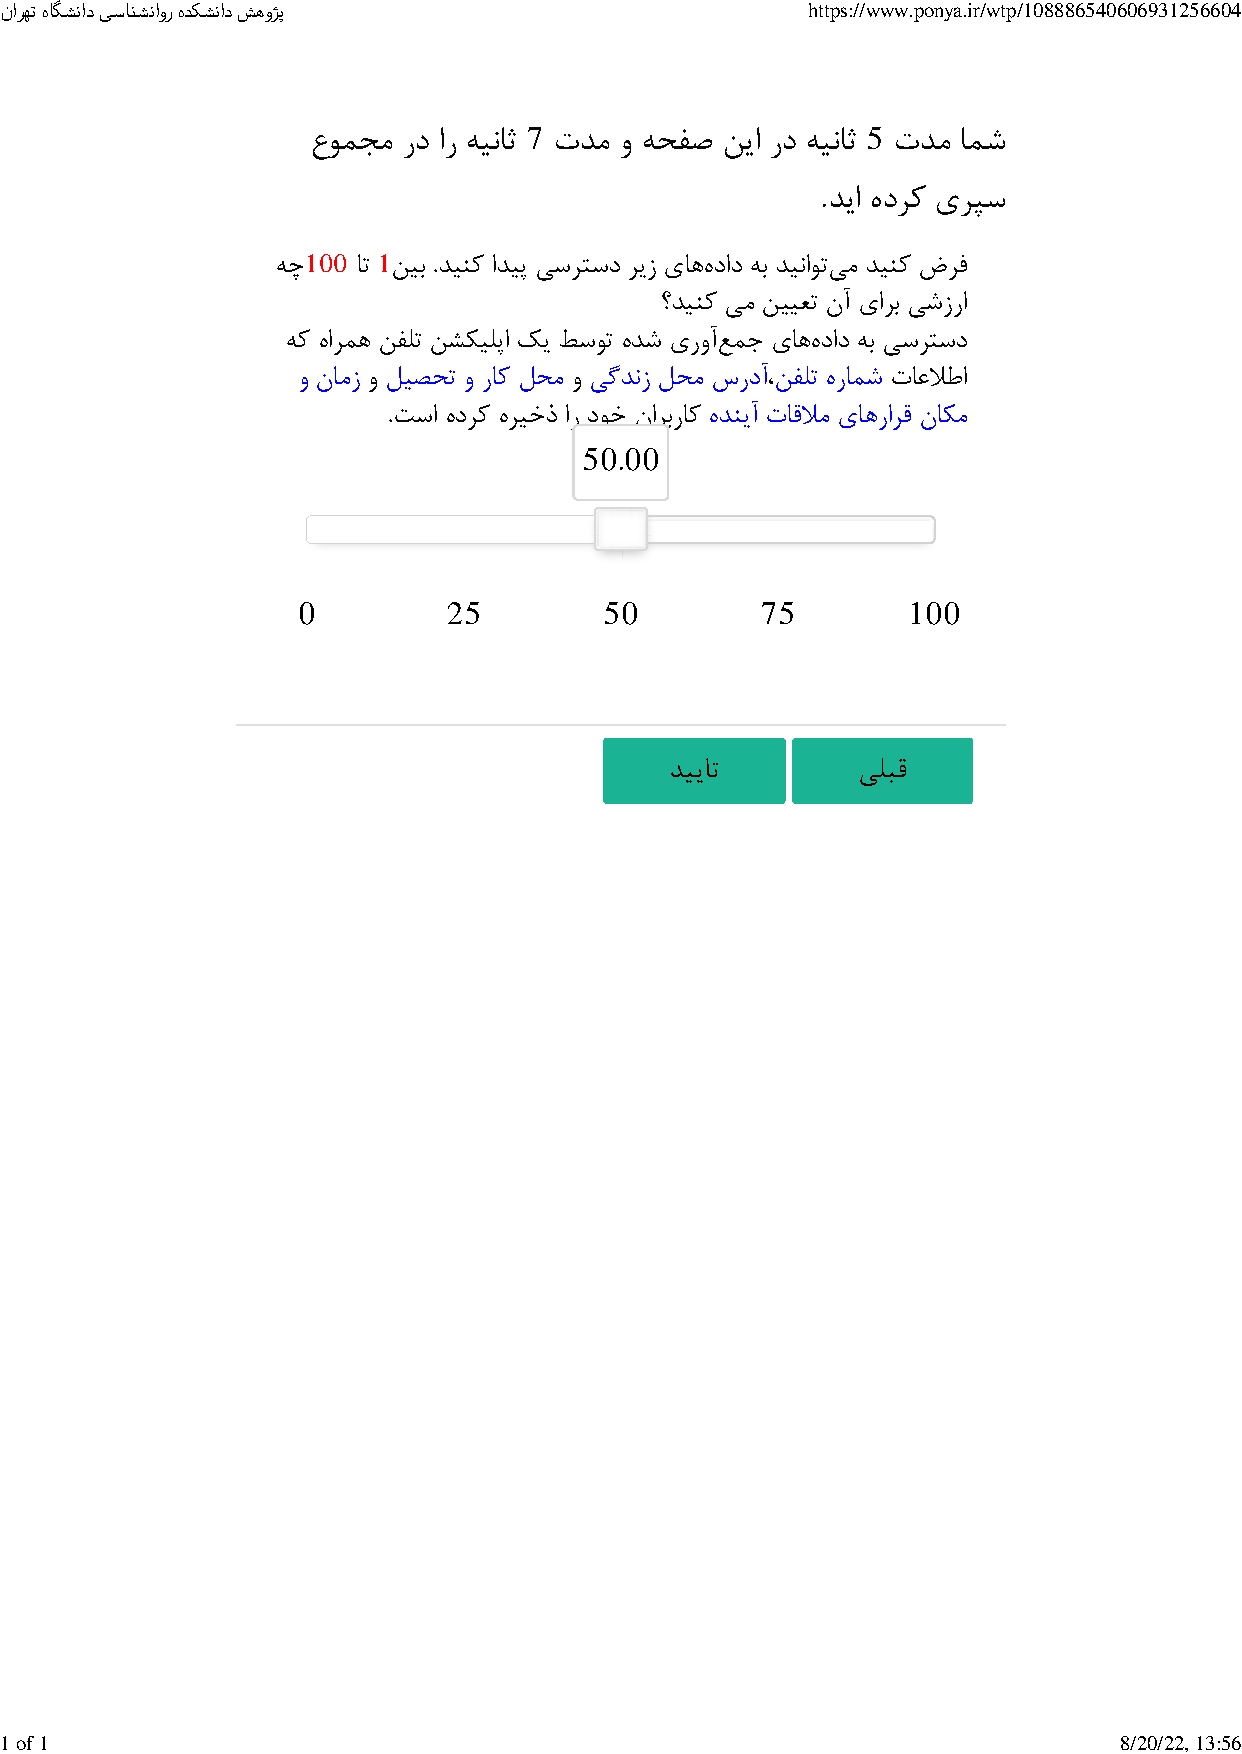
\includepdf[pages={1}]{./questionnares/wtp.pdf}
\begin{figure}[htpb]
    \centering
    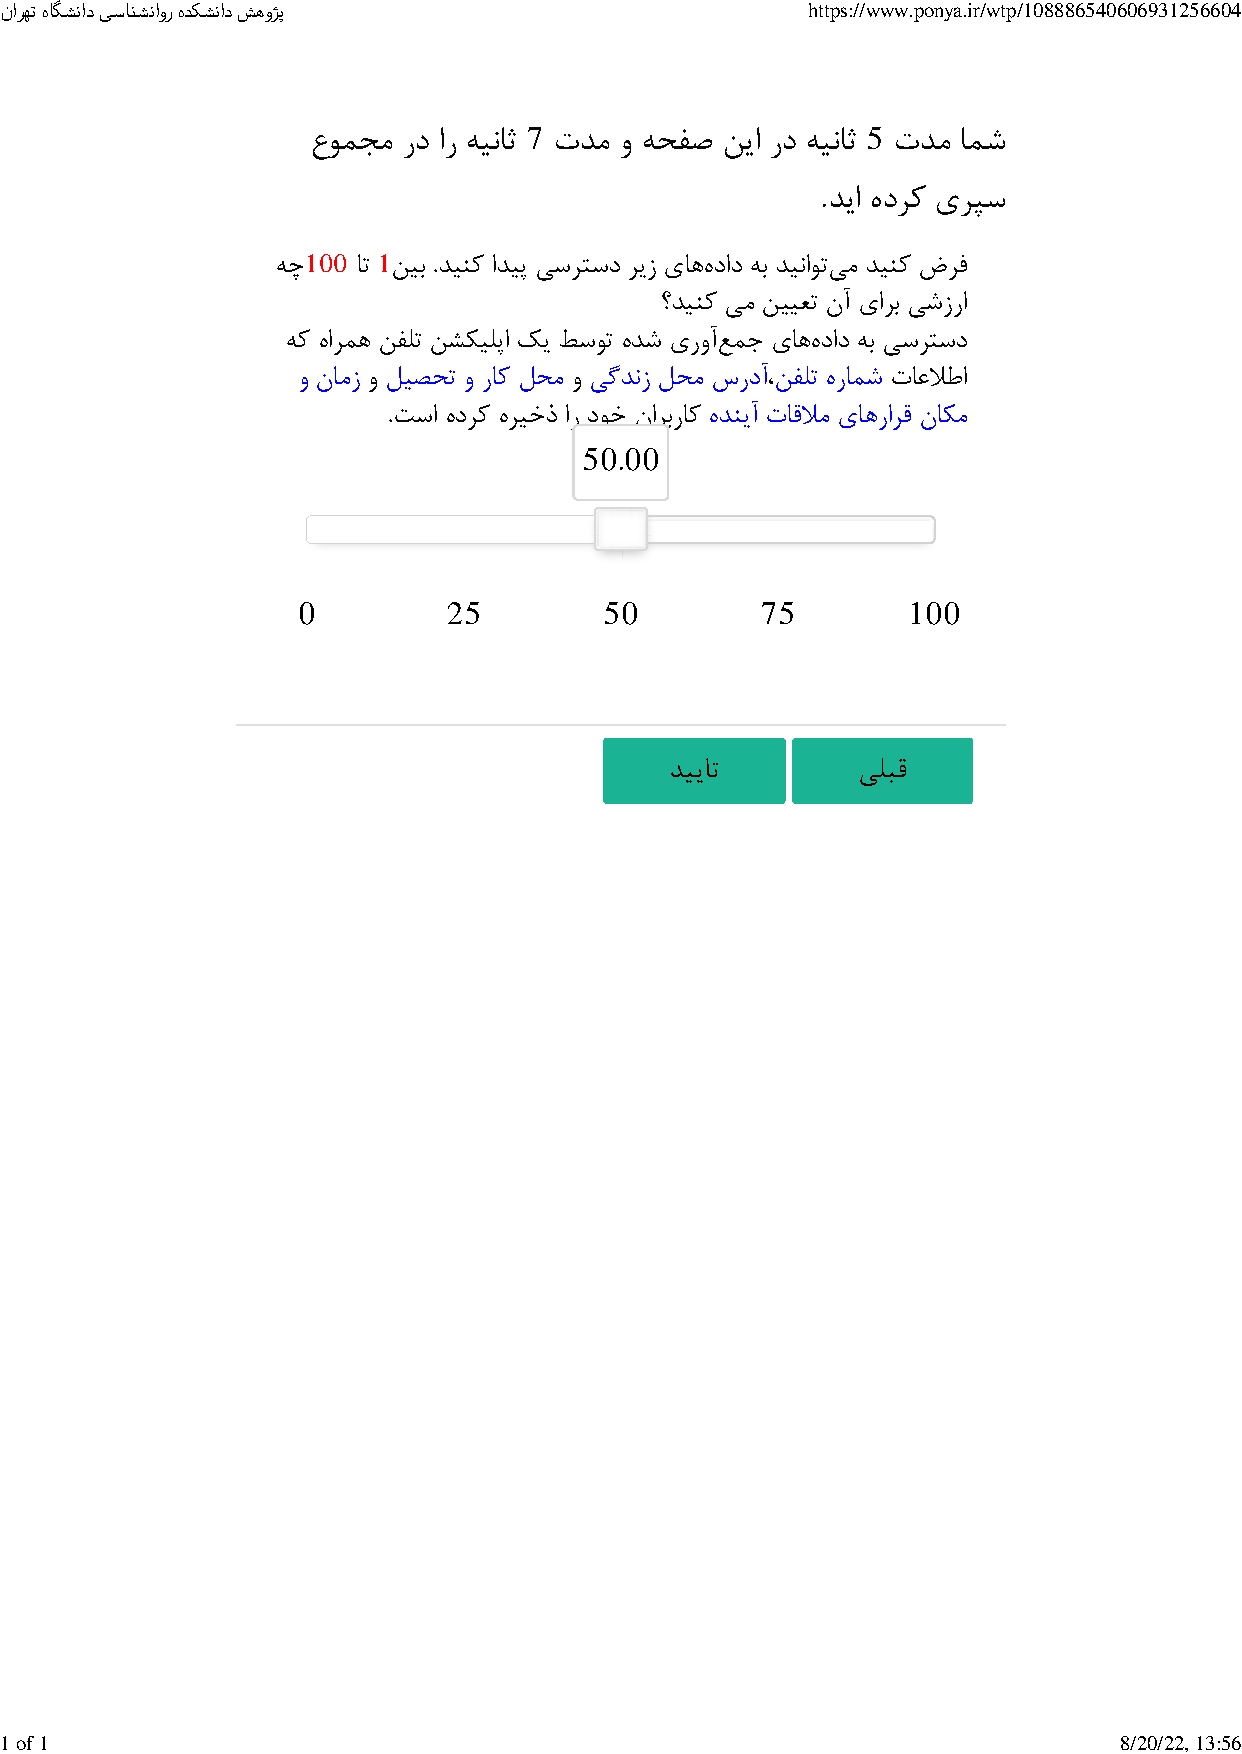
\includegraphics[width=0.8\textwidth]{./questionnares/wtp.pdf}
    \caption{The first page of the \texttt{tikz} reference manual.}
    \label{fig:tikzpgf}
\end{figure}
پرسشنامه ۲


\chapter{ابزار مبتنی بر وب}
\begin{figure}[htpb]
    \centering
    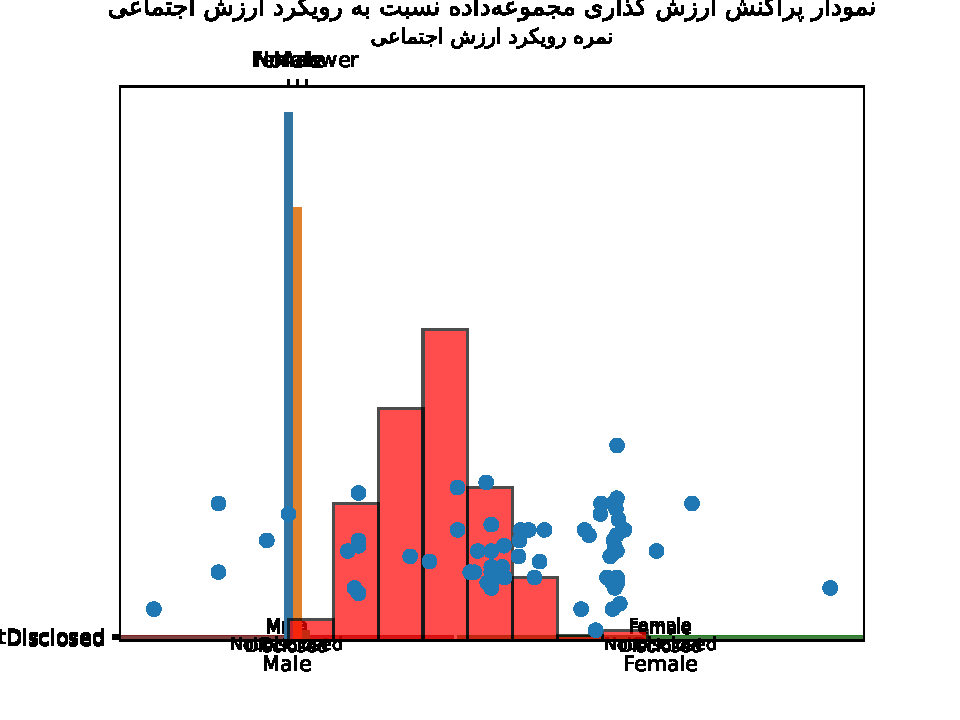
\includegraphics[width=0.8\textwidth]{./img/ScatterSVOScoreDarkTriadScore.pdf}
    \caption{نمودار پراکنش نمره رویکرد ارزش اجتماعی را نسبت به نمره سه‌گانه تاریک نشان می دهد. }
    \label{fig:ScatterSVOScoreDarkTriadScore}
\end{figure}
شکل 
\label{fig:sexualityAndSVOAgainstPopulation}



 % ^ %%%% 
\begin{figure}[htpb]
\centering
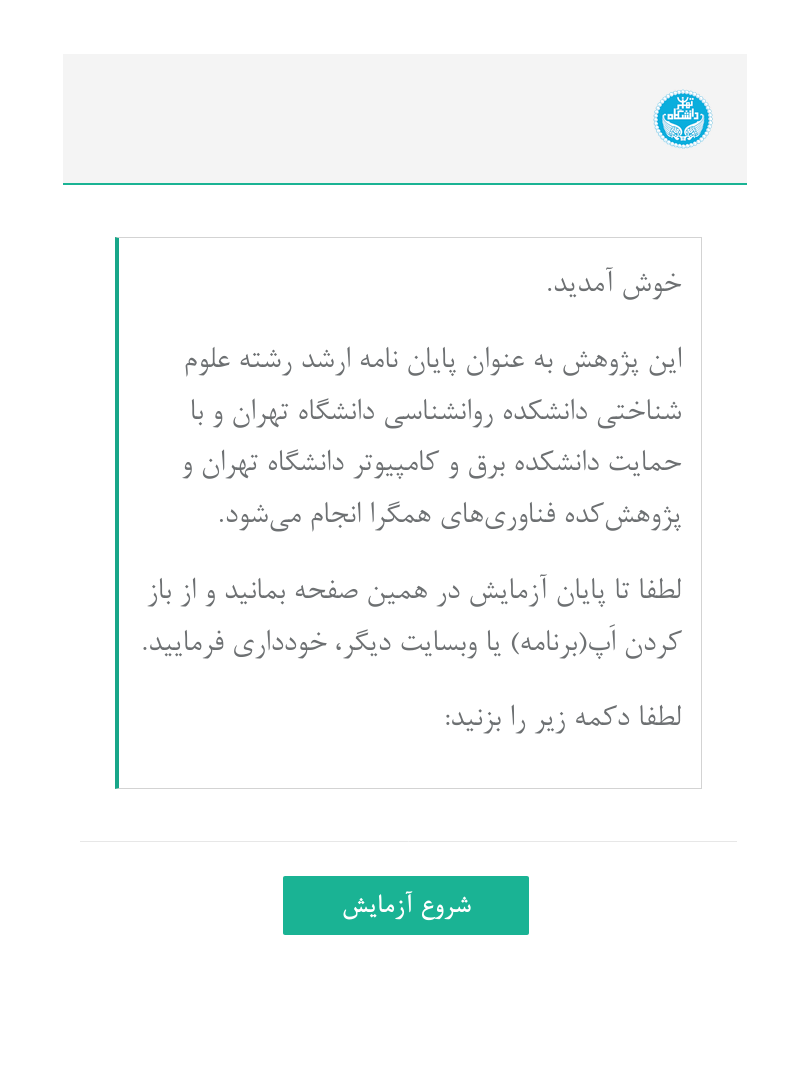
\includegraphics[width=0.8\textwidth,height=0.8\textheight,keepaspectratio]{./img/Task1.png}
\caption{ صفحه 1 آزمایش }
\label{fig:Task1}
\end{figure}
 
 
 % ^ %%%% 
\begin{figure}[htpb]
\centering
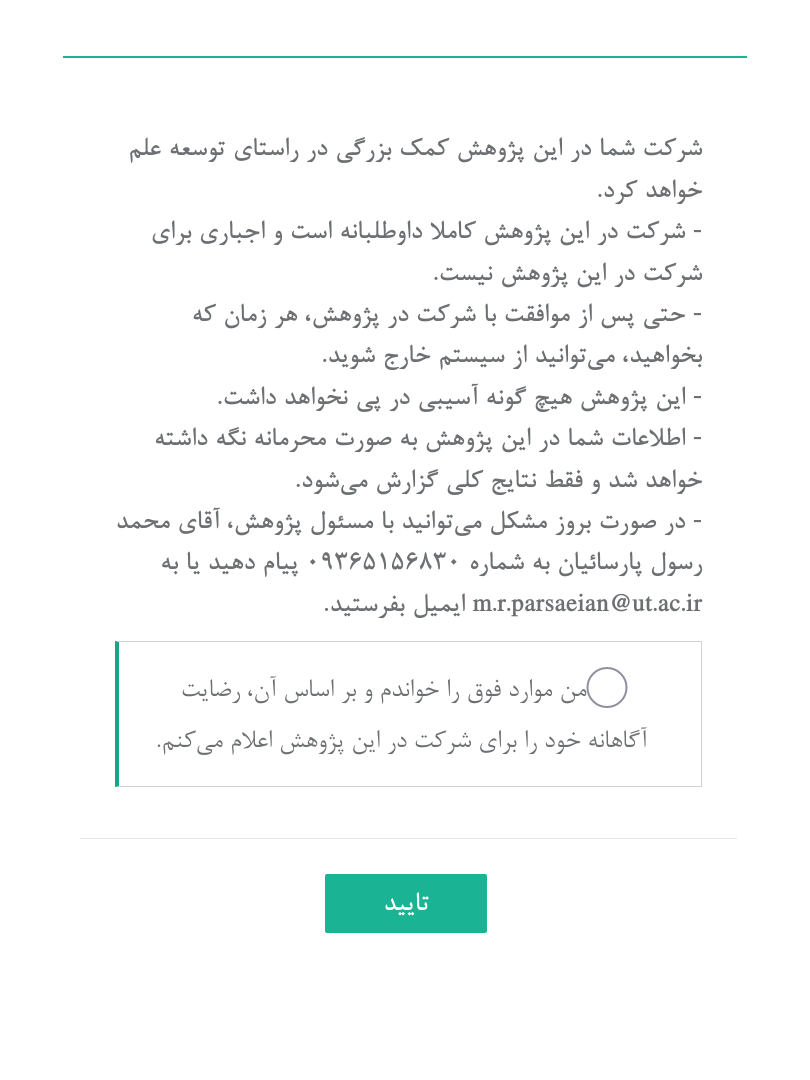
\includegraphics[width=0.8\textwidth,height=0.8\textheight,keepaspectratio]{./img/Task2.png}
\caption{ صفحه 2 آزمایش }
\label{fig:Task2}
\end{figure}
 
 
 % ^ %%%% 
\begin{figure}[htpb]
\centering
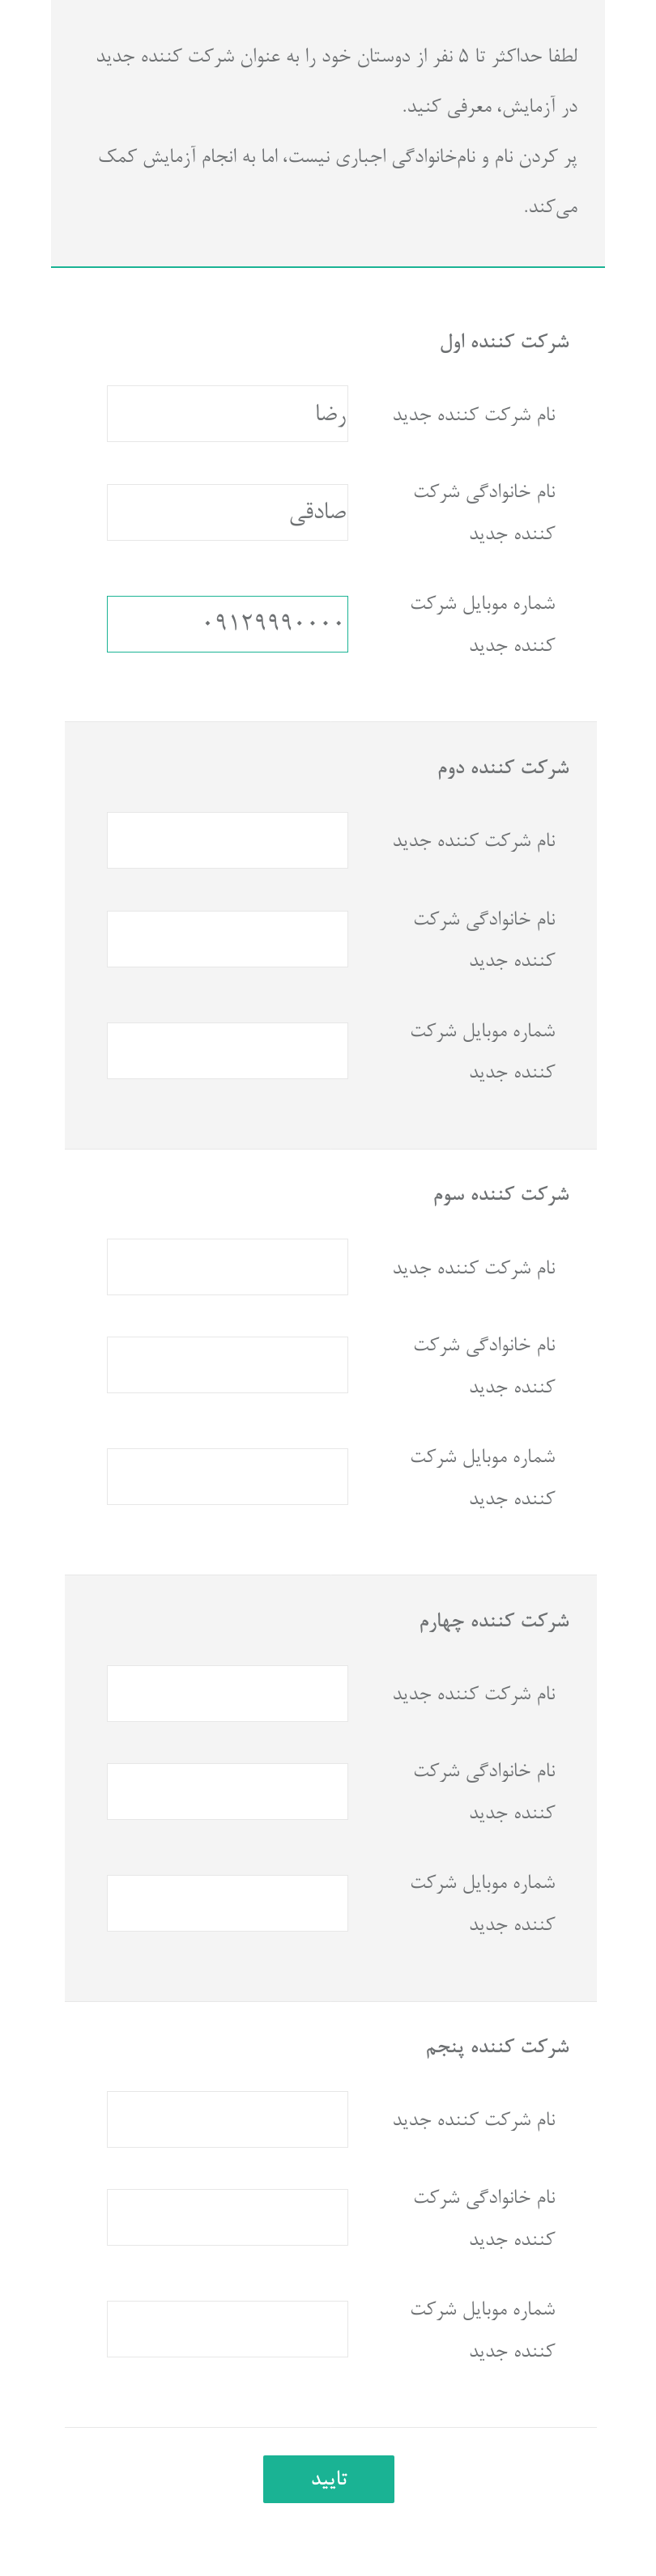
\includegraphics[width=0.8\textwidth,height=0.8\textheight,keepaspectratio]{./img/Task3.png}
\caption{ صفحه 3 آزمایش }
\label{fig:Task3}
\end{figure}
 
 
 % ^ %%%% 
\begin{figure}[htpb]
\centering
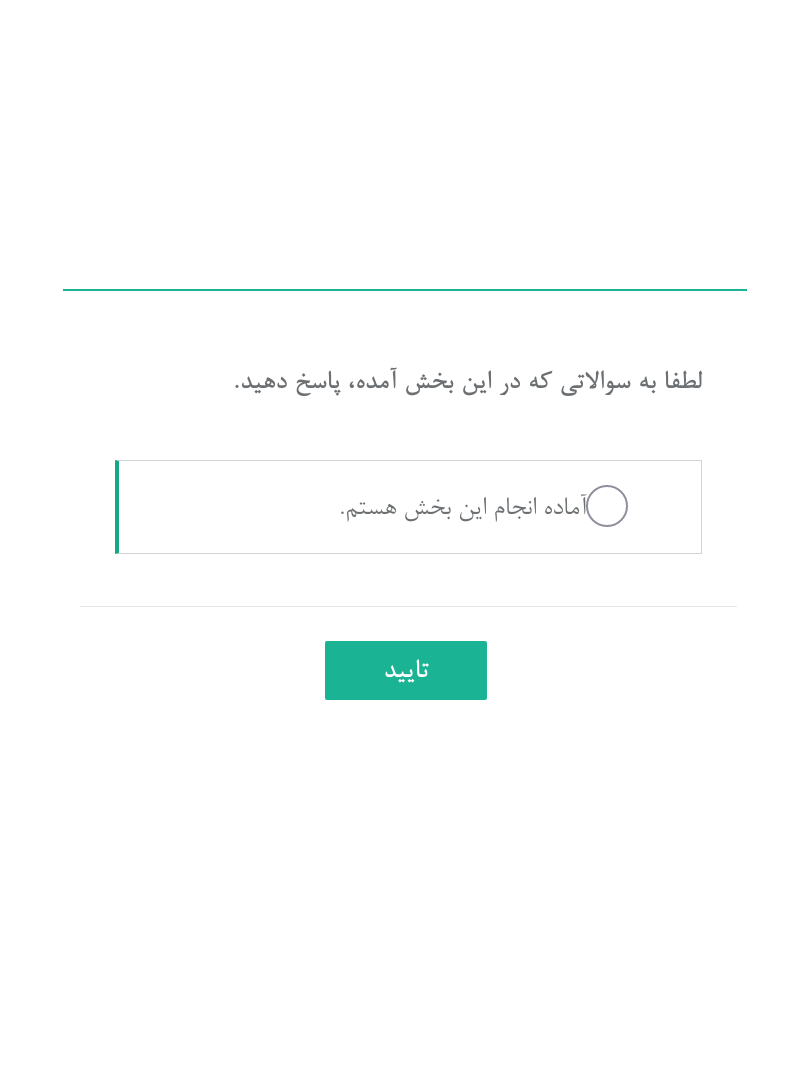
\includegraphics[width=0.8\textwidth,height=0.8\textheight,keepaspectratio]{./img/Task4.png}
\caption{ صفحه 4 آزمایش }
\label{fig:Task4}
\end{figure}
 
 
 % ^ %%%% 
\begin{figure}[htpb]
\centering
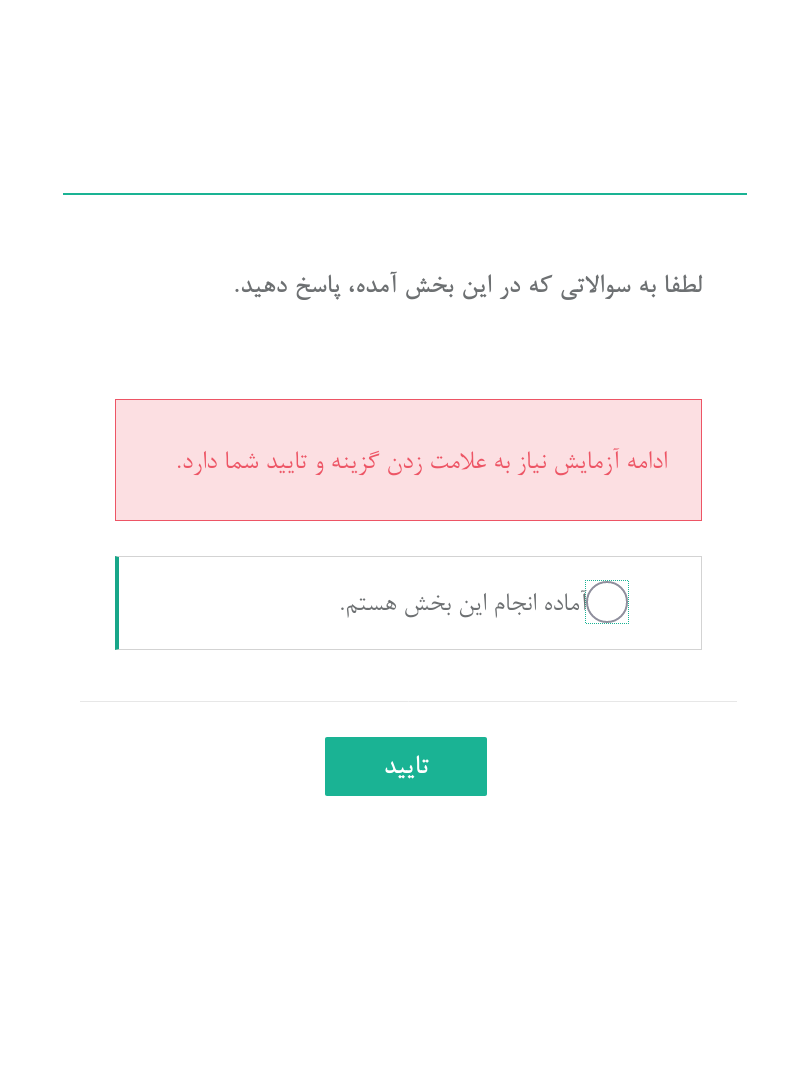
\includegraphics[width=0.8\textwidth,height=0.8\textheight,keepaspectratio]{./img/Task5.png}
\caption{ صفحه 5 آزمایش }
\label{fig:Task5}
\end{figure}
 
 
 % ^ %%%% 
\begin{figure}[htpb]
\centering
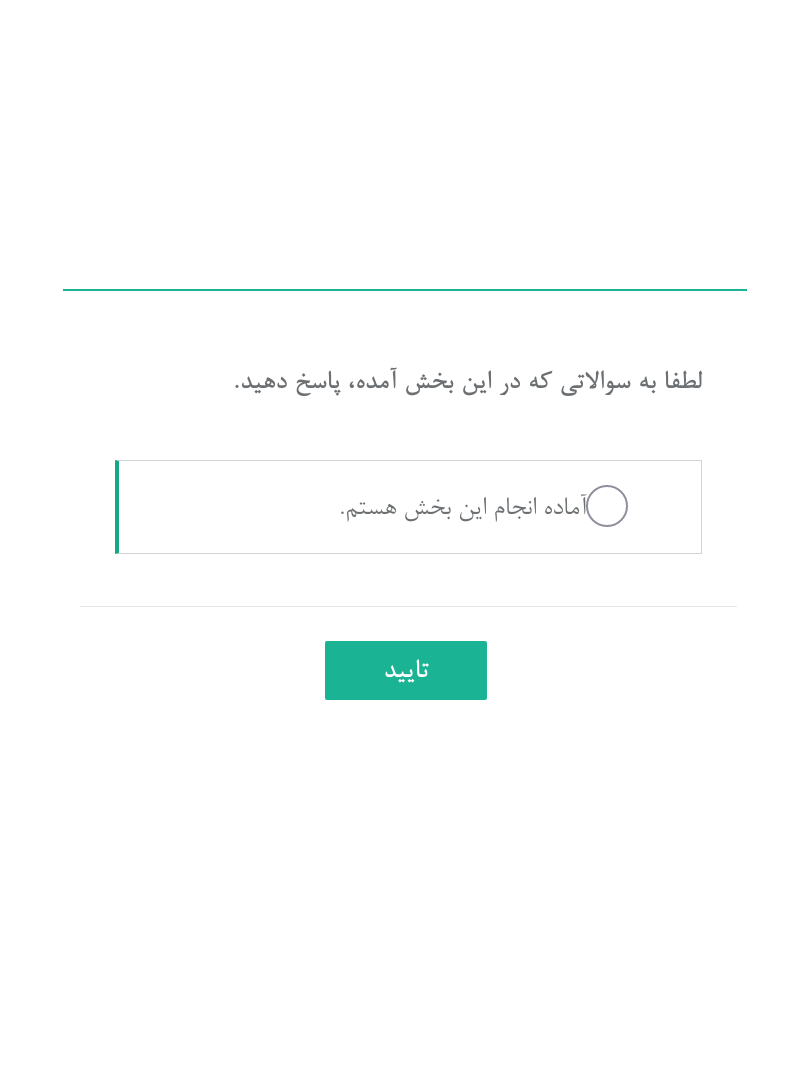
\includegraphics[width=0.8\textwidth,height=0.8\textheight,keepaspectratio]{./img/Task6.png}
\caption{ صفحه 6 آزمایش }
\label{fig:Task6}
\end{figure}
 
 
 % ^ %%%% 
\begin{figure}[htpb]
\centering
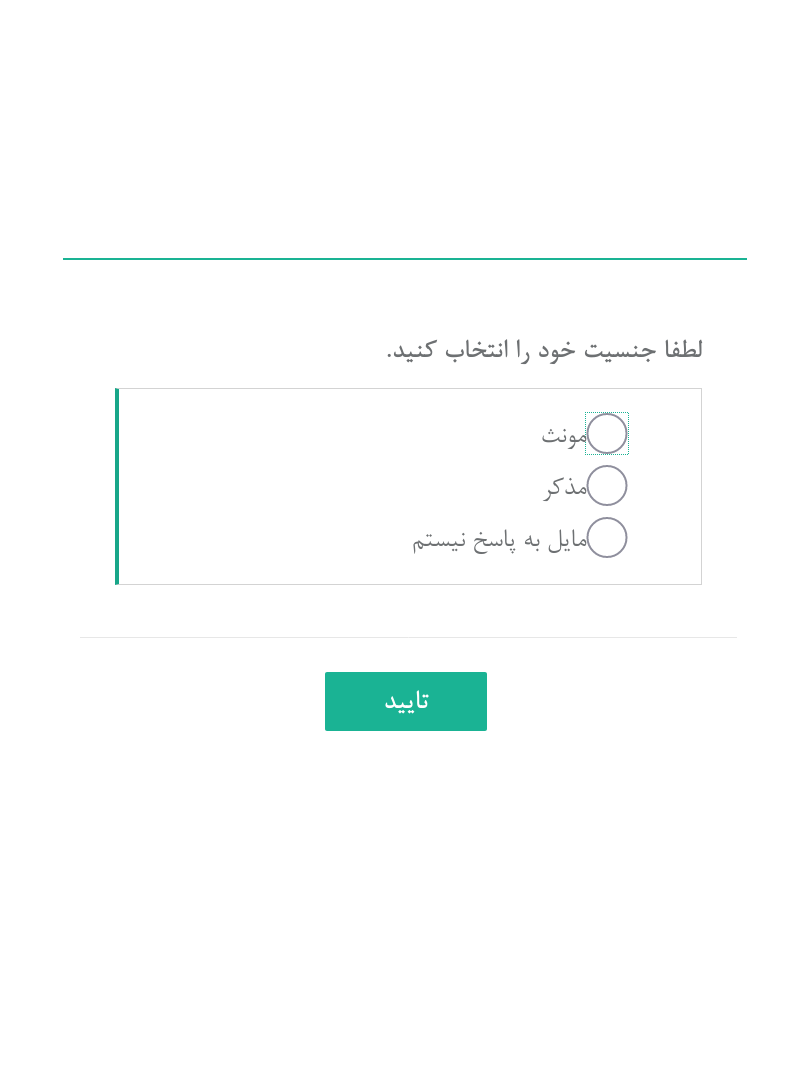
\includegraphics[width=0.8\textwidth,height=0.8\textheight,keepaspectratio]{./img/Task7.png}
\caption{ صفحه 7 آزمایش }
\label{fig:Task7}
\end{figure}
 
 
 % ^ %%%% 
\begin{figure}[htpb]
\centering
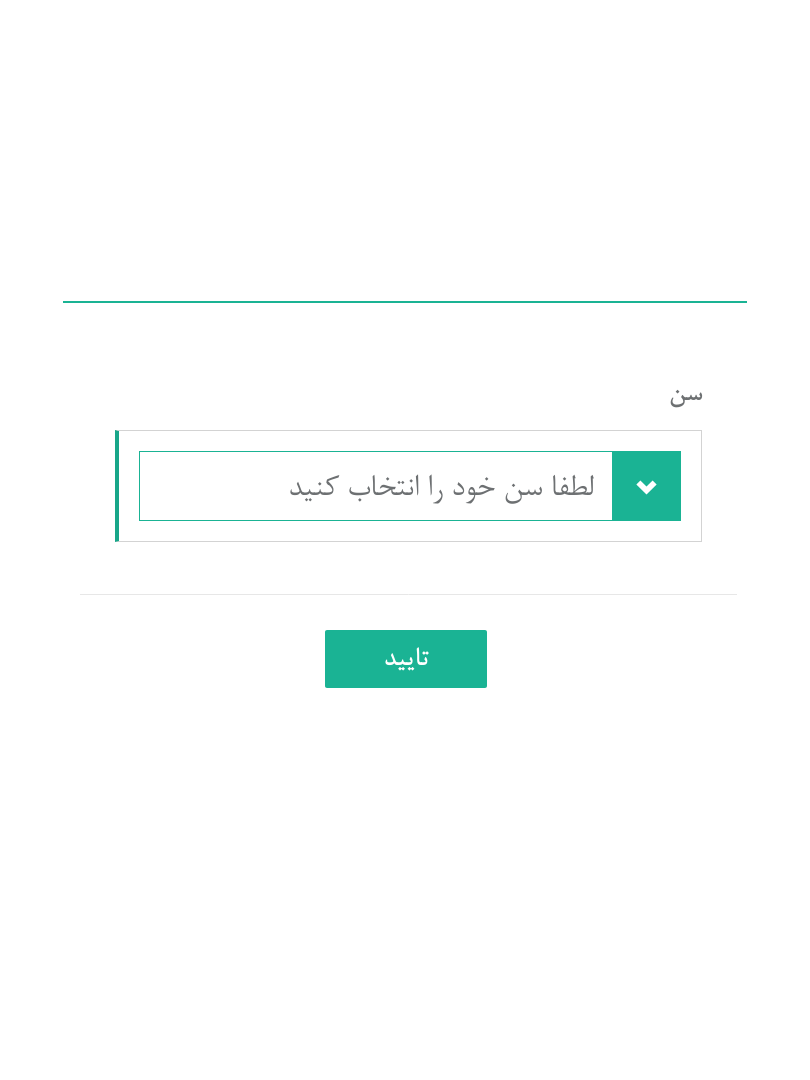
\includegraphics[width=0.8\textwidth,height=0.8\textheight,keepaspectratio]{./img/Task8.png}
\caption{ صفحه 8 آزمایش }
\label{fig:Task8}
\end{figure}
 
 
 % ^ %%%% 
\begin{figure}[htpb]
\centering
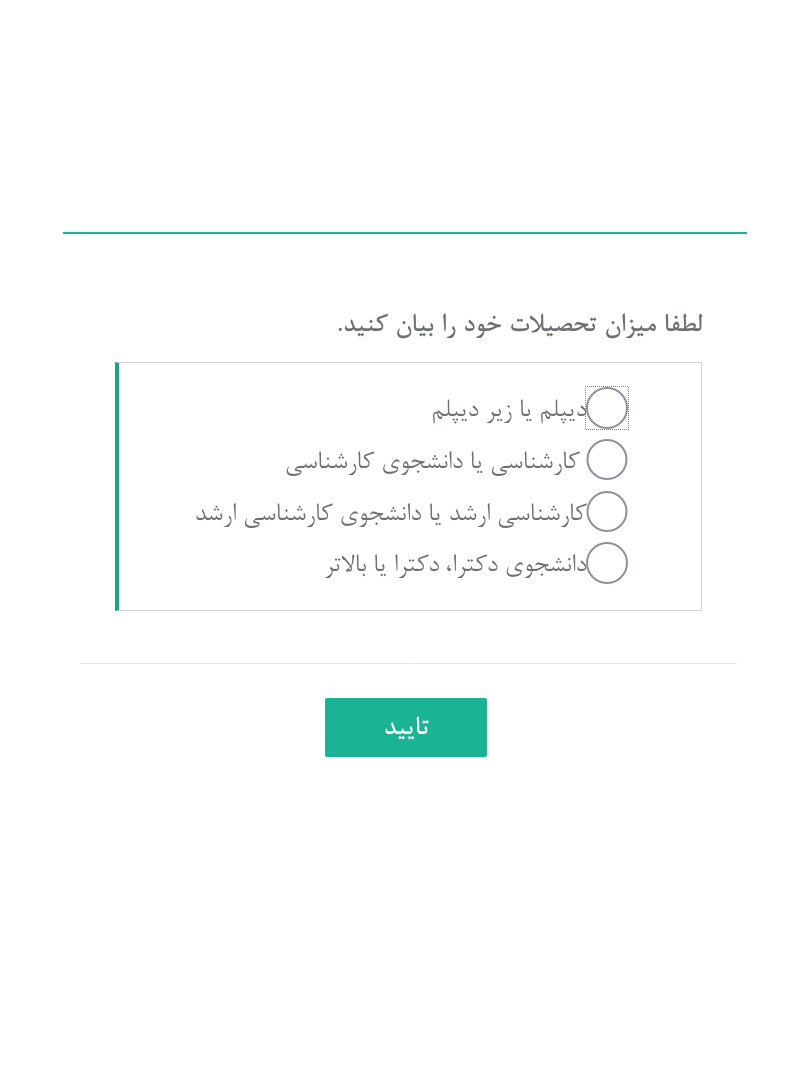
\includegraphics[width=0.8\textwidth,height=0.8\textheight,keepaspectratio]{./img/Task9.png}
\caption{ صفحه 9 آزمایش }
\label{fig:Task9}
\end{figure}
 
 
 % ^ %%%% 
\begin{figure}[htpb]
\centering
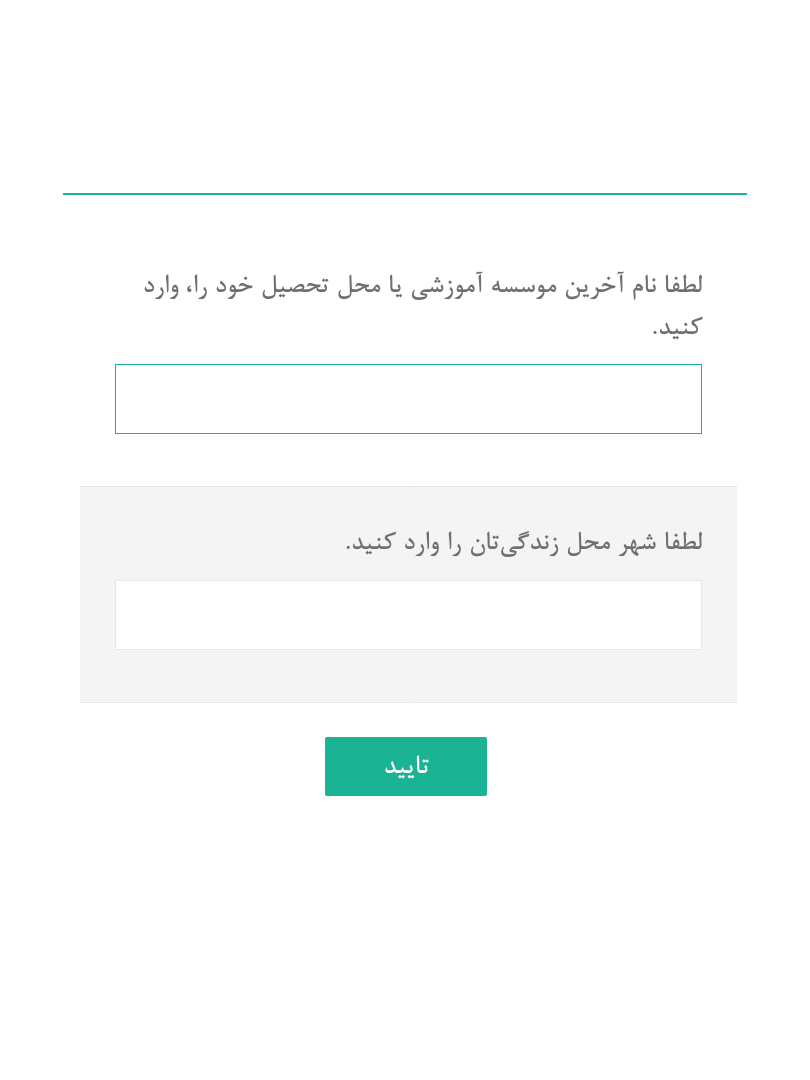
\includegraphics[width=0.8\textwidth,height=0.8\textheight,keepaspectratio]{./img/Task10.png}
\caption{ صفحه 10 آزمایش }
\label{fig:Task10}
\end{figure}
 
 
 % ^ %%%% 
\begin{figure}[htpb]
\centering
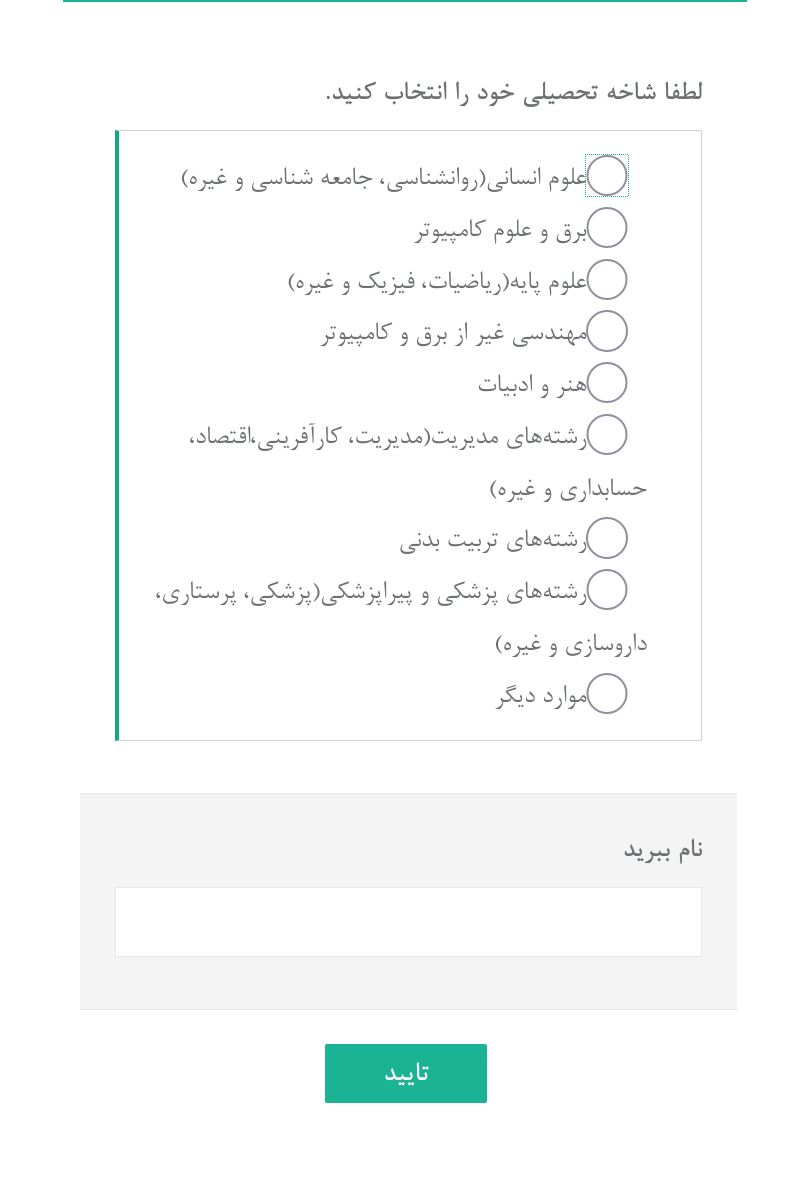
\includegraphics[width=0.8\textwidth,height=0.8\textheight,keepaspectratio]{./img/Task11.png}
\caption{ صفحه 11 آزمایش }
\label{fig:Task11}
\end{figure}
 
 
 % ^ %%%% 
\begin{figure}[htpb]
\centering
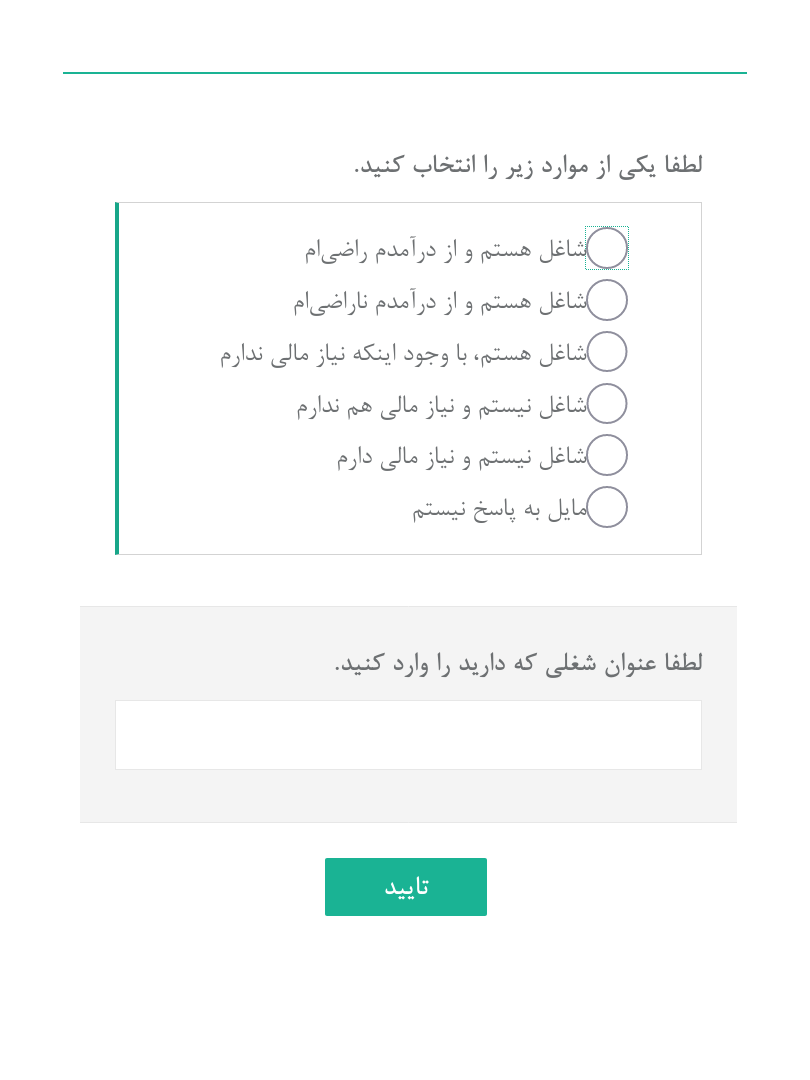
\includegraphics[width=0.8\textwidth,height=0.8\textheight,keepaspectratio]{./img/Task12.png}
\caption{ صفحه 12 آزمایش }
\label{fig:Task12}
\end{figure}
 
 
 % ^ %%%% 
\begin{figure}[htpb]
\centering
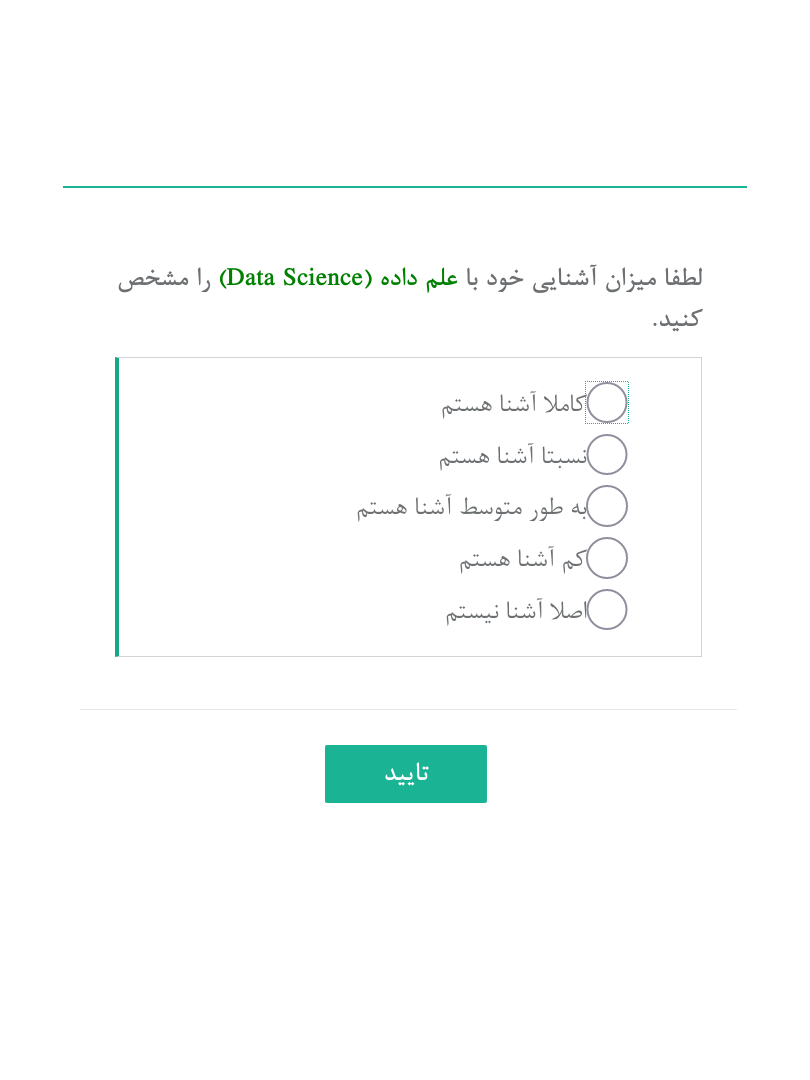
\includegraphics[width=0.8\textwidth,height=0.8\textheight,keepaspectratio]{./img/Task13.png}
\caption{ صفحه 13 آزمایش }
\label{fig:Task13}
\end{figure}
 
 
 % ^ %%%% 
\begin{figure}[htpb]
\centering
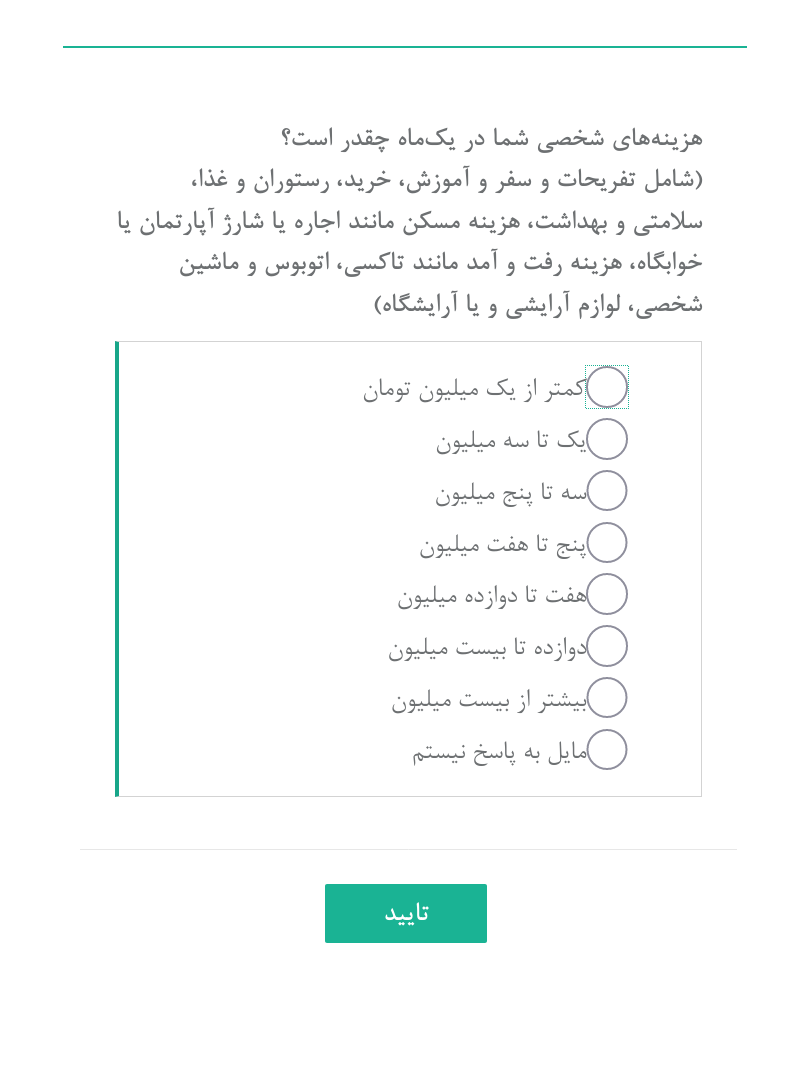
\includegraphics[width=0.8\textwidth,height=0.8\textheight,keepaspectratio]{./img/Task14.png}
\caption{ صفحه 14 آزمایش }
\label{fig:Task14}
\end{figure}
 
 
 % ^ %%%% 
\begin{figure}[htpb]
\centering
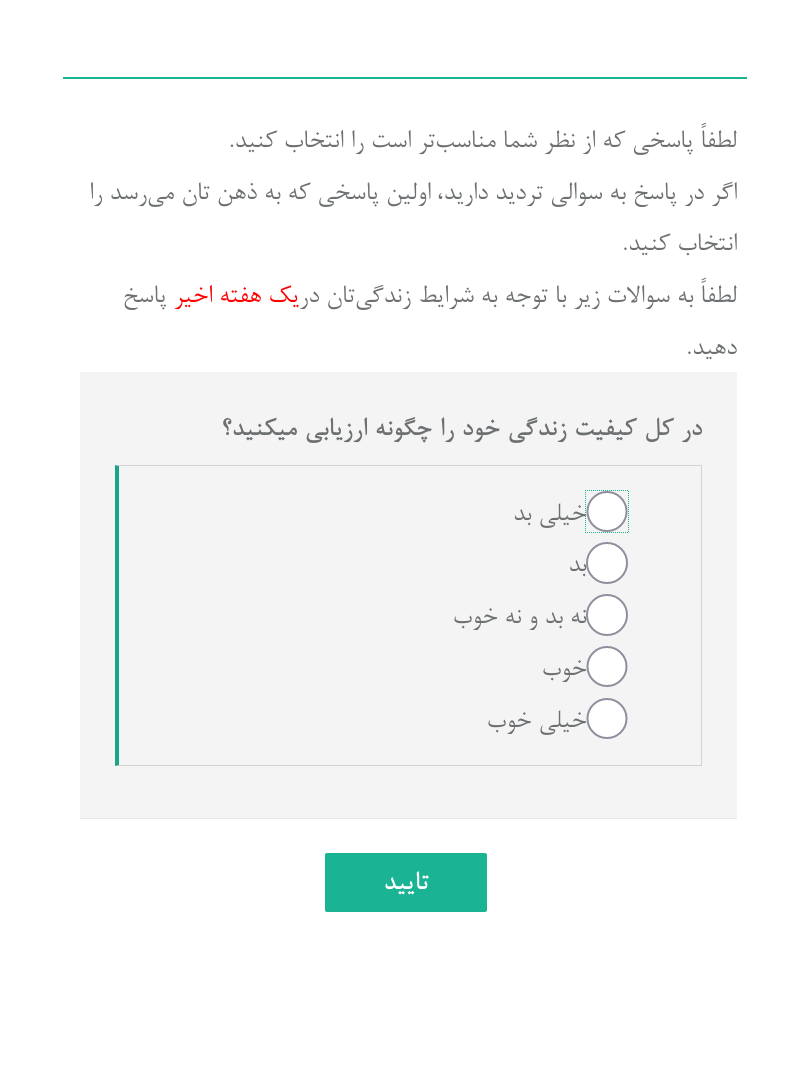
\includegraphics[width=0.8\textwidth,height=0.8\textheight,keepaspectratio]{./img/Task15.png}
\caption{ صفحه 15 آزمایش }
\label{fig:Task15}
\end{figure}
 
 
 % ^ %%%% 
\begin{figure}[htpb]
\centering
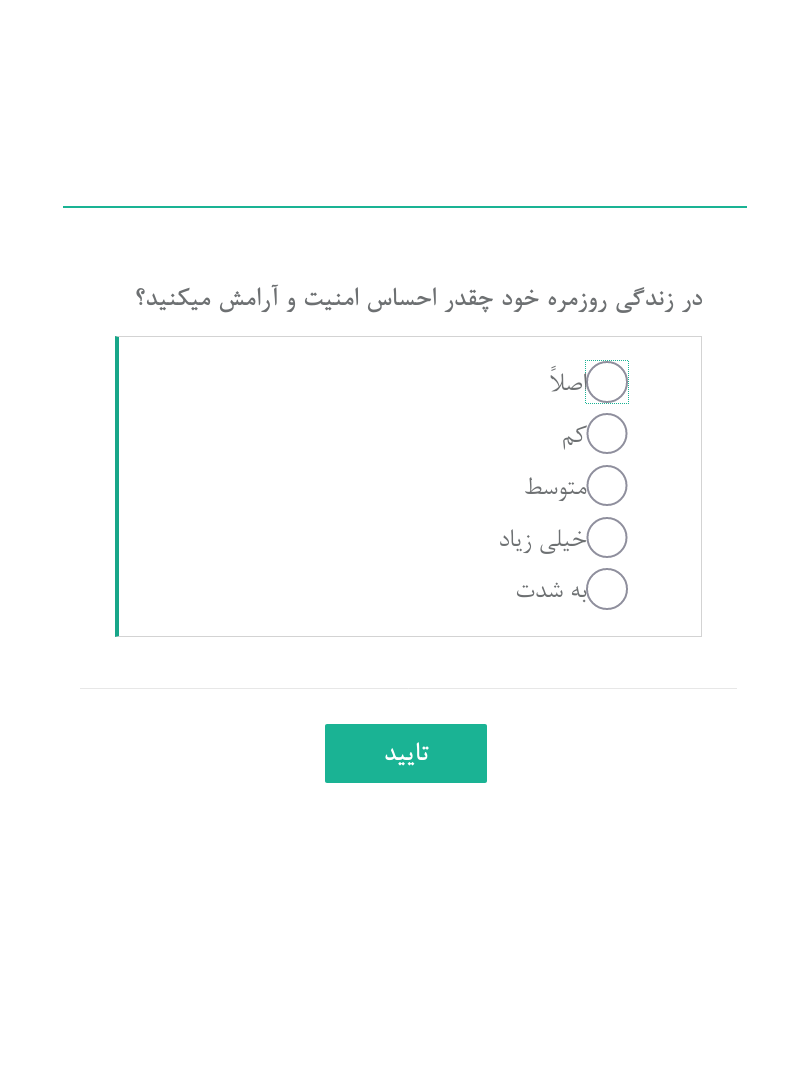
\includegraphics[width=0.8\textwidth,height=0.8\textheight,keepaspectratio]{./img/Task16.png}
\caption{ صفحه 16 آزمایش }
\label{fig:Task16}
\end{figure}
 
 
 % ^ %%%% 
\begin{figure}[htpb]
\centering
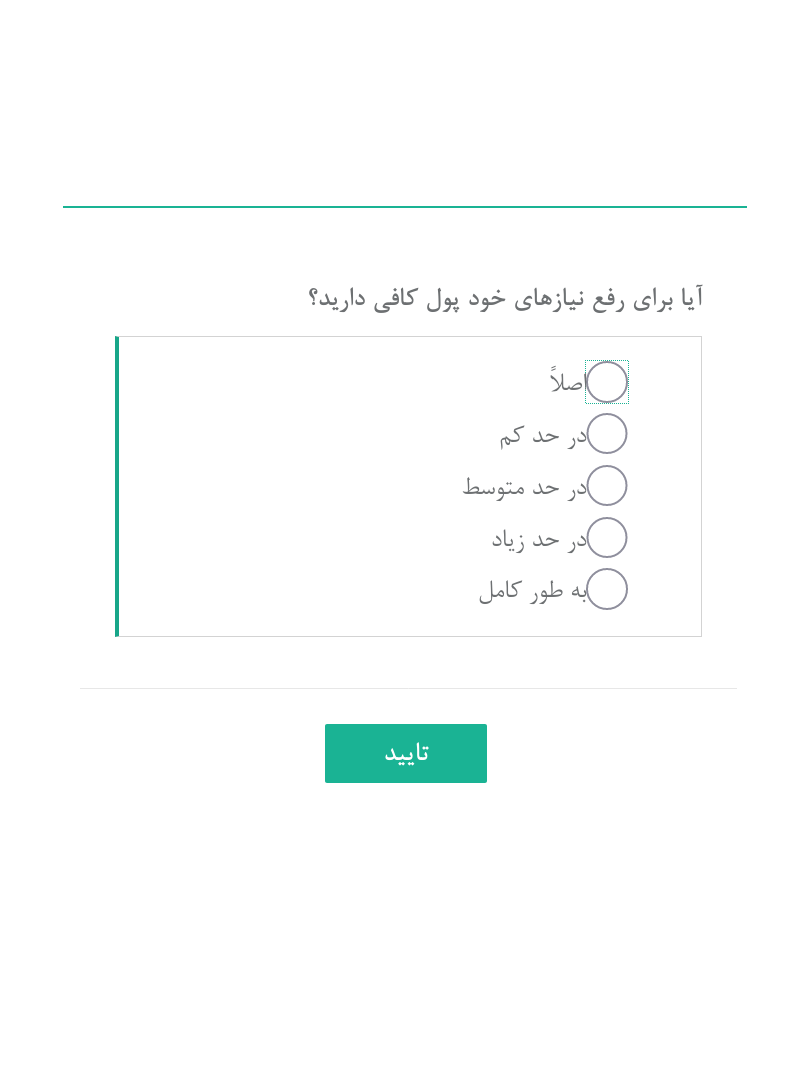
\includegraphics[width=0.8\textwidth,height=0.8\textheight,keepaspectratio]{./img/Task17.png}
\caption{ صفحه 17 آزمایش }
\label{fig:Task17}
\end{figure}
 
 
 % ^ %%%% 
\begin{figure}[htpb]
\centering
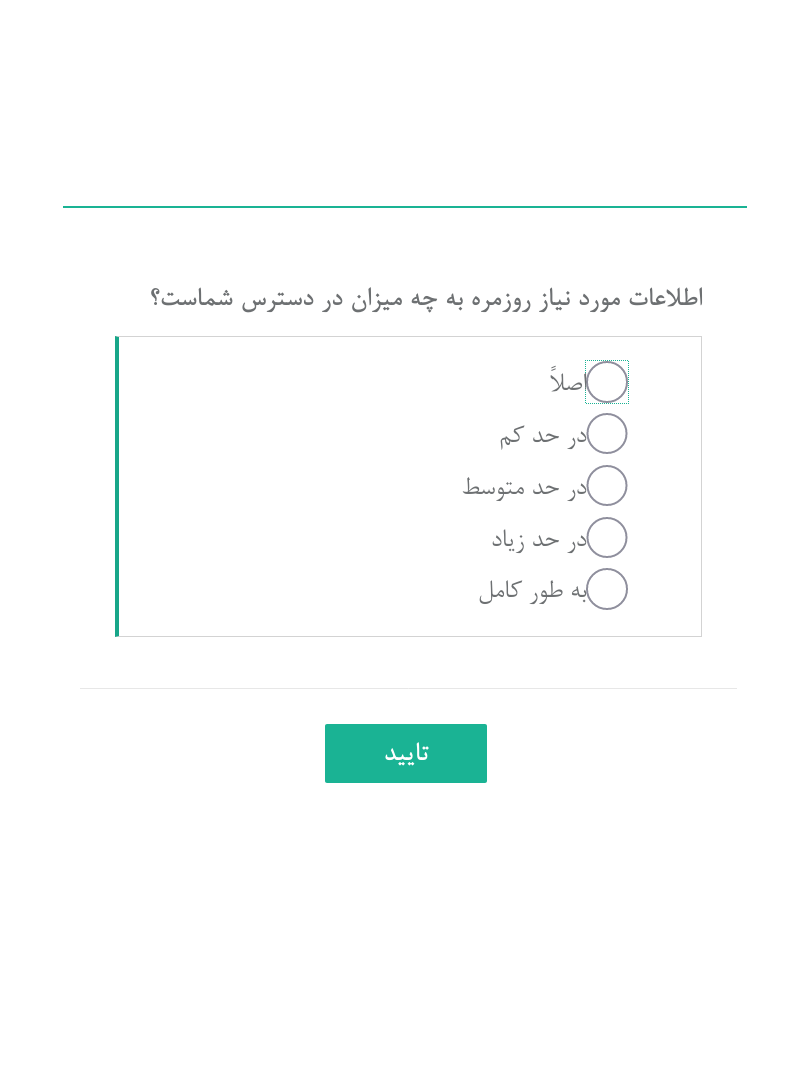
\includegraphics[width=0.8\textwidth,height=0.8\textheight,keepaspectratio]{./img/Task18.png}
\caption{ صفحه 18 آزمایش }
\label{fig:Task18}
\end{figure}
 
 
 % ^ %%%% 
\begin{figure}[htpb]
\centering
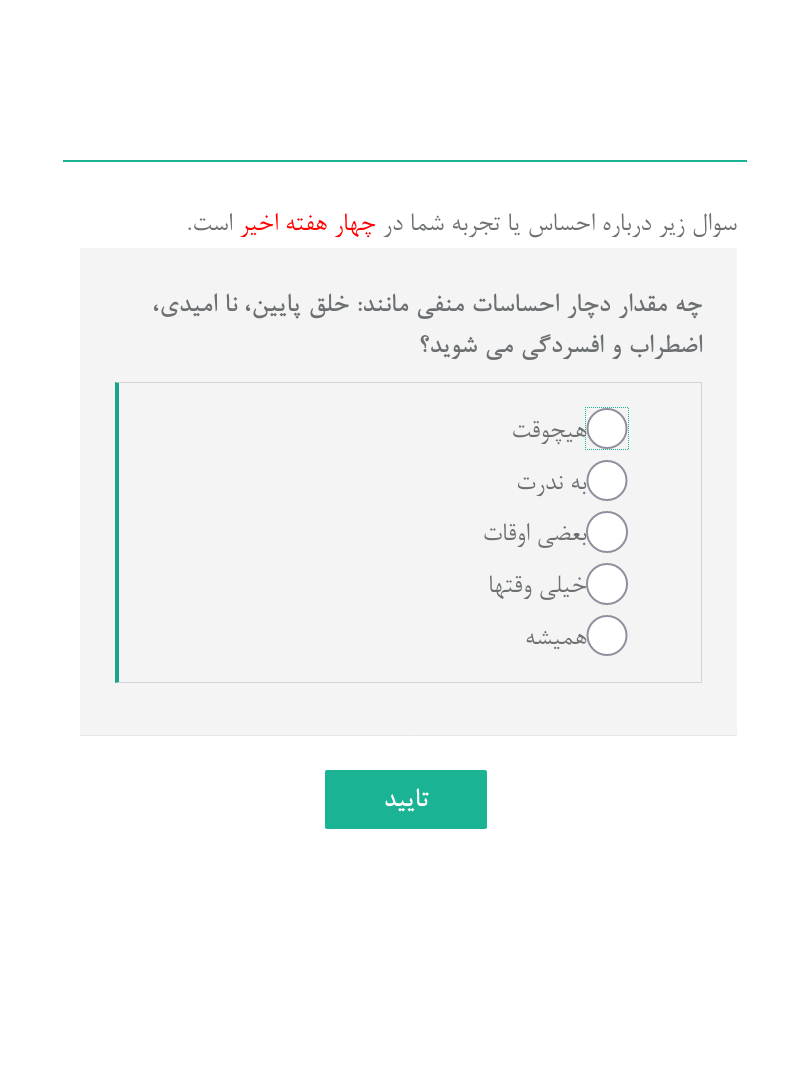
\includegraphics[width=0.8\textwidth,height=0.8\textheight,keepaspectratio]{./img/Task19.png}
\caption{ صفحه 19 آزمایش }
\label{fig:Task19}
\end{figure}
 
 
 % ^ %%%% 
\begin{figure}[htpb]
\centering
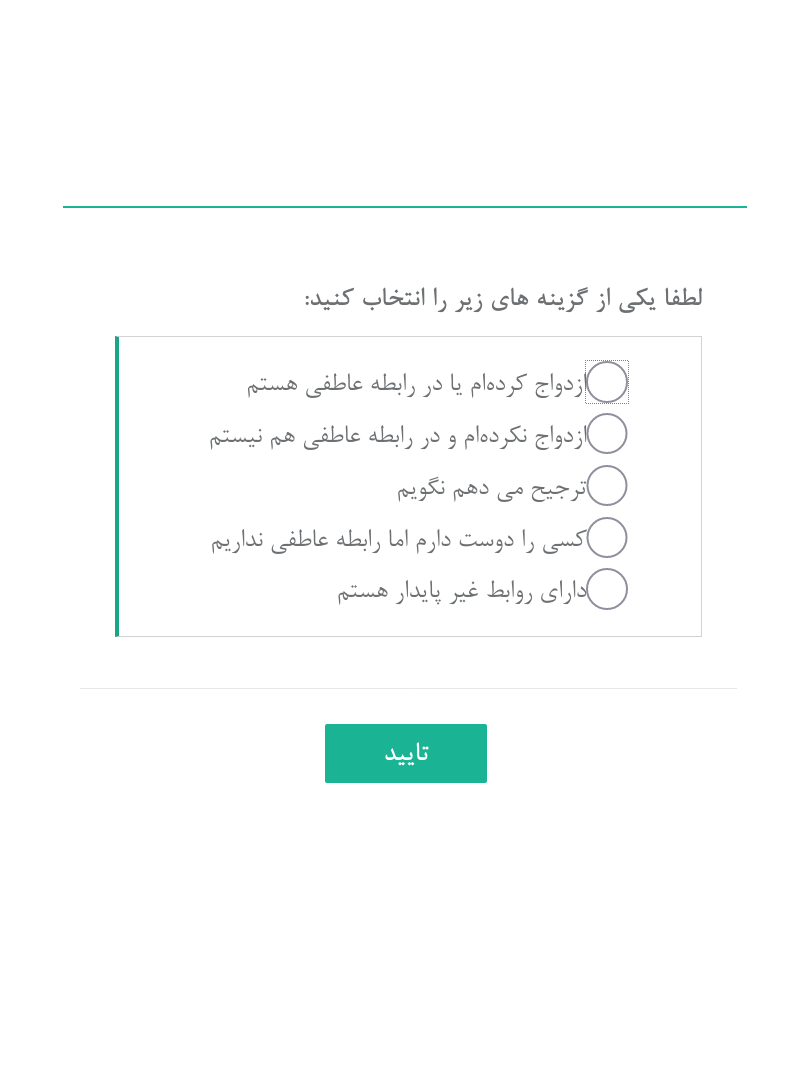
\includegraphics[width=0.8\textwidth,height=0.8\textheight,keepaspectratio]{./img/Task20.png}
\caption{ صفحه 20 آزمایش }
\label{fig:Task20}
\end{figure}
 
 
 % ^ %%%% 
\begin{figure}[htpb]
\centering
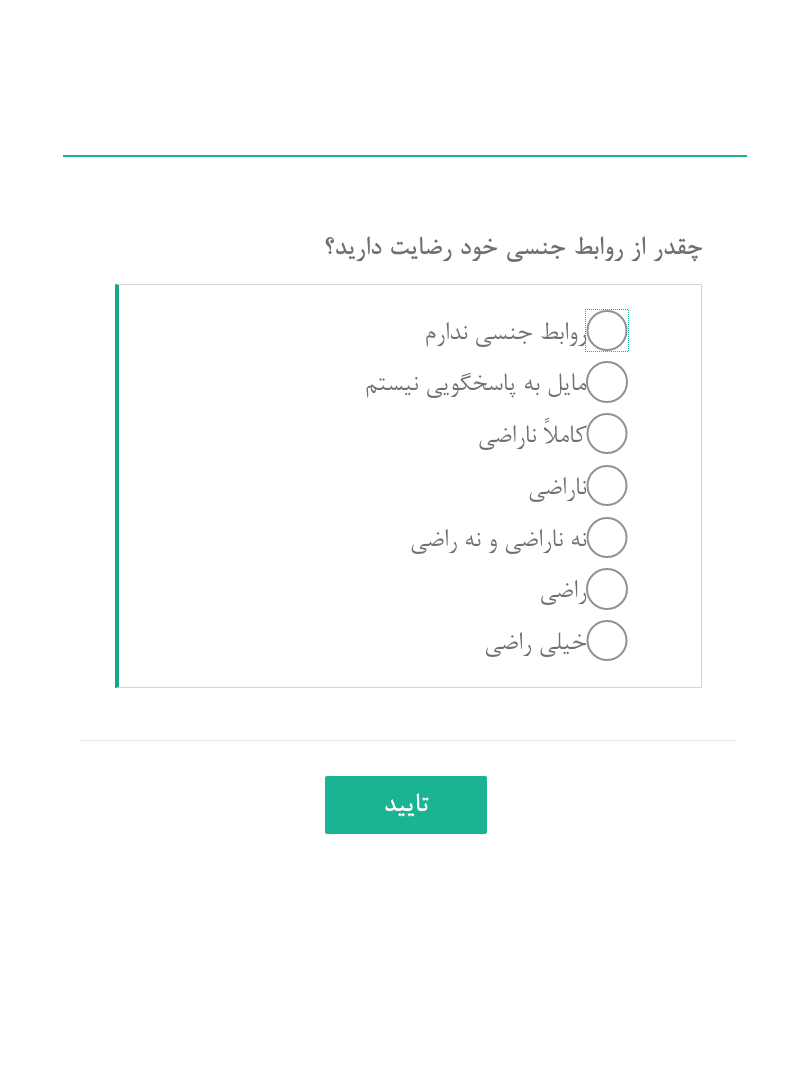
\includegraphics[width=0.8\textwidth,height=0.8\textheight,keepaspectratio]{./img/Task21.png}
\caption{ صفحه 21 آزمایش }
\label{fig:Task21}
\end{figure}
 
 
 % ^ %%%% 
\begin{figure}[htpb]
\centering
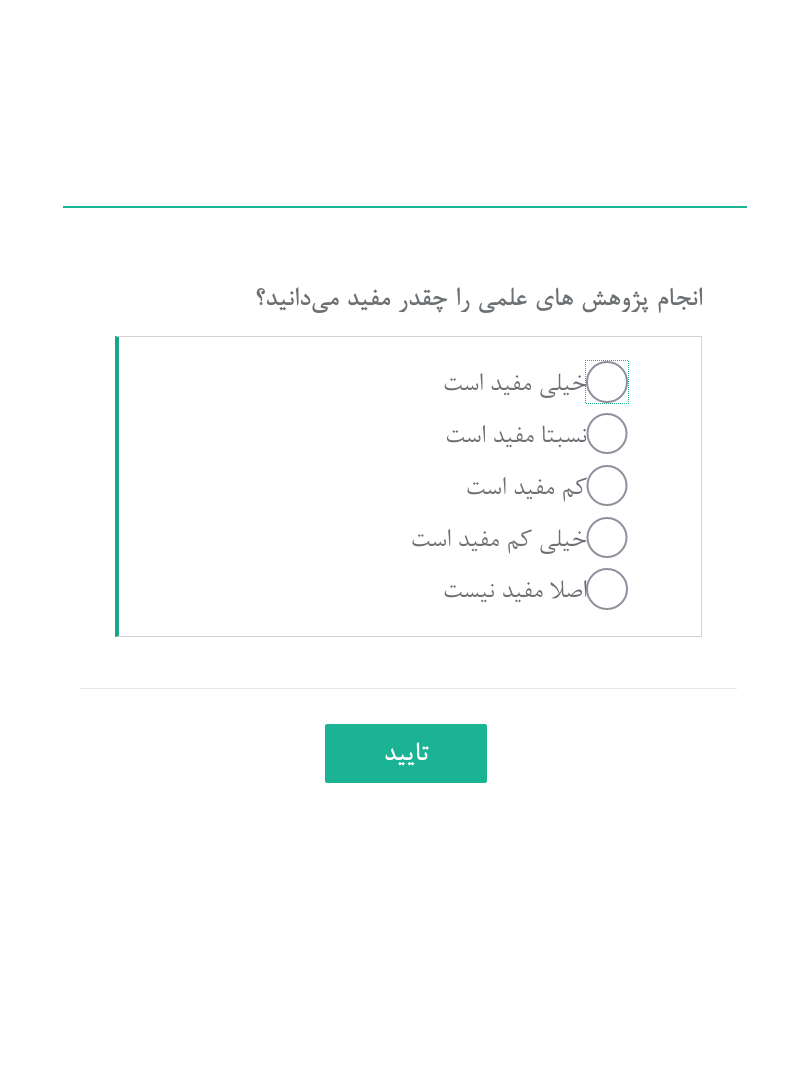
\includegraphics[width=0.8\textwidth,height=0.8\textheight,keepaspectratio]{./img/Task22.png}
\caption{ صفحه 22 آزمایش }
\label{fig:Task22}
\end{figure}
 
 
 % ^ %%%% 
\begin{figure}[htpb]
\centering
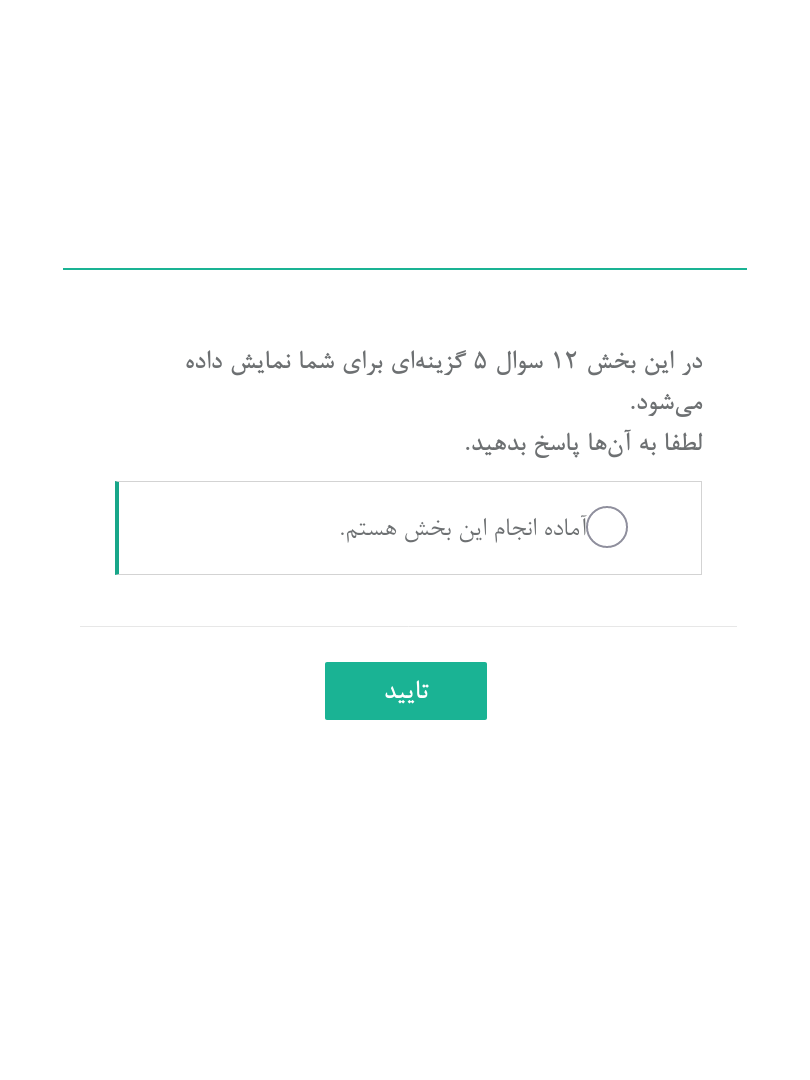
\includegraphics[width=0.8\textwidth,height=0.8\textheight,keepaspectratio]{./img/Task23.png}
\caption{ صفحه 23 آزمایش }
\label{fig:Task23}
\end{figure}
 
 
 % ^ %%%% 
\begin{figure}[htpb]
\centering
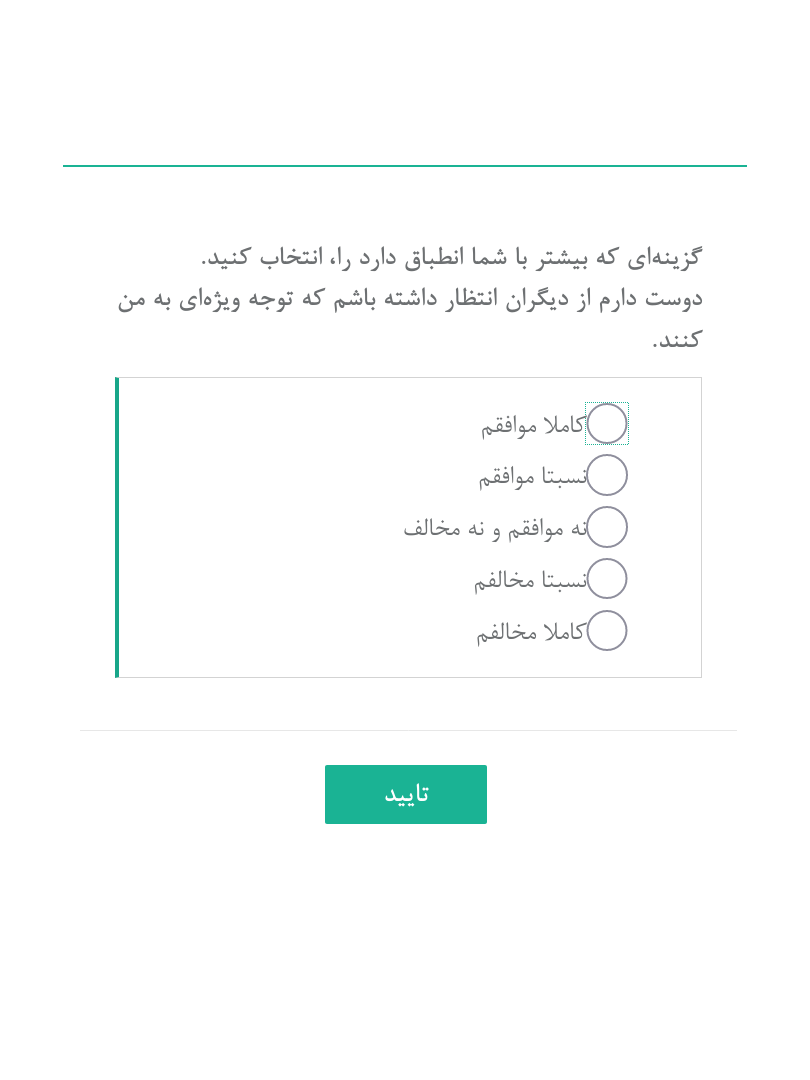
\includegraphics[width=0.8\textwidth,height=0.8\textheight,keepaspectratio]{./img/Task24.png}
\caption{ صفحه 24 آزمایش }
\label{fig:Task24}
\end{figure}
 
 
 % ^ %%%% 
\begin{figure}[htpb]
\centering
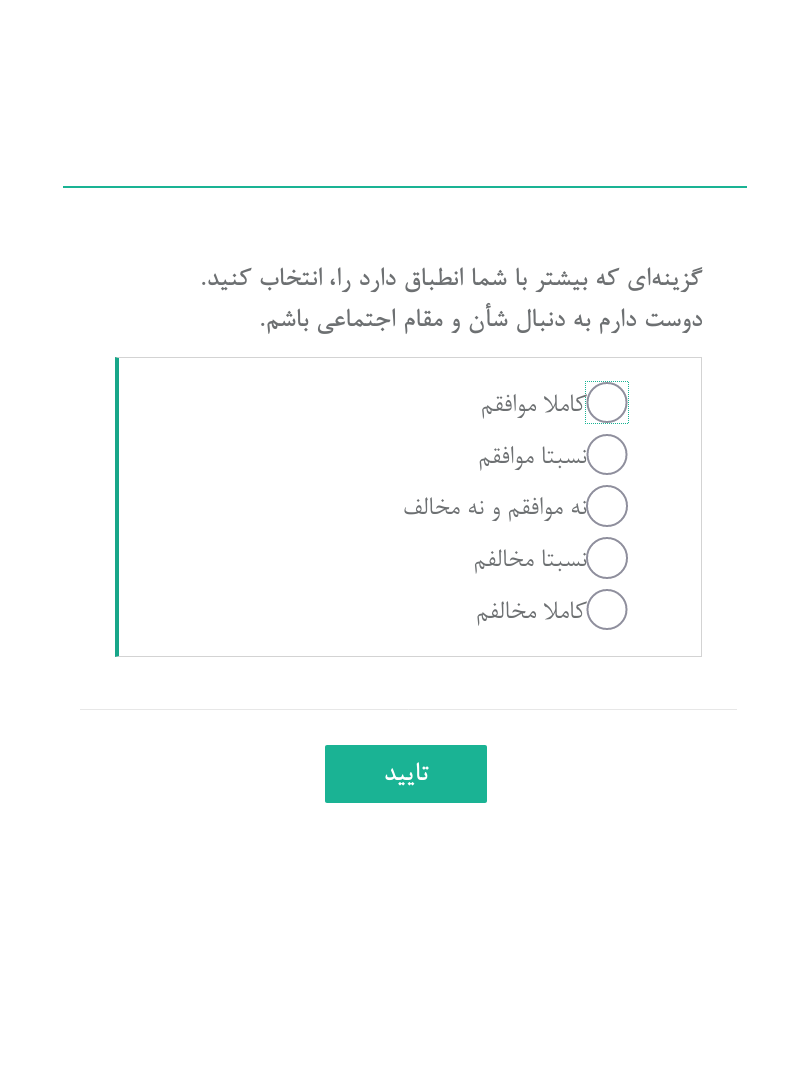
\includegraphics[width=0.8\textwidth,height=0.8\textheight,keepaspectratio]{./img/Task25.png}
\caption{ صفحه 25 آزمایش }
\label{fig:Task25}
\end{figure}
 
 
 % ^ %%%% 
\begin{figure}[htpb]
\centering
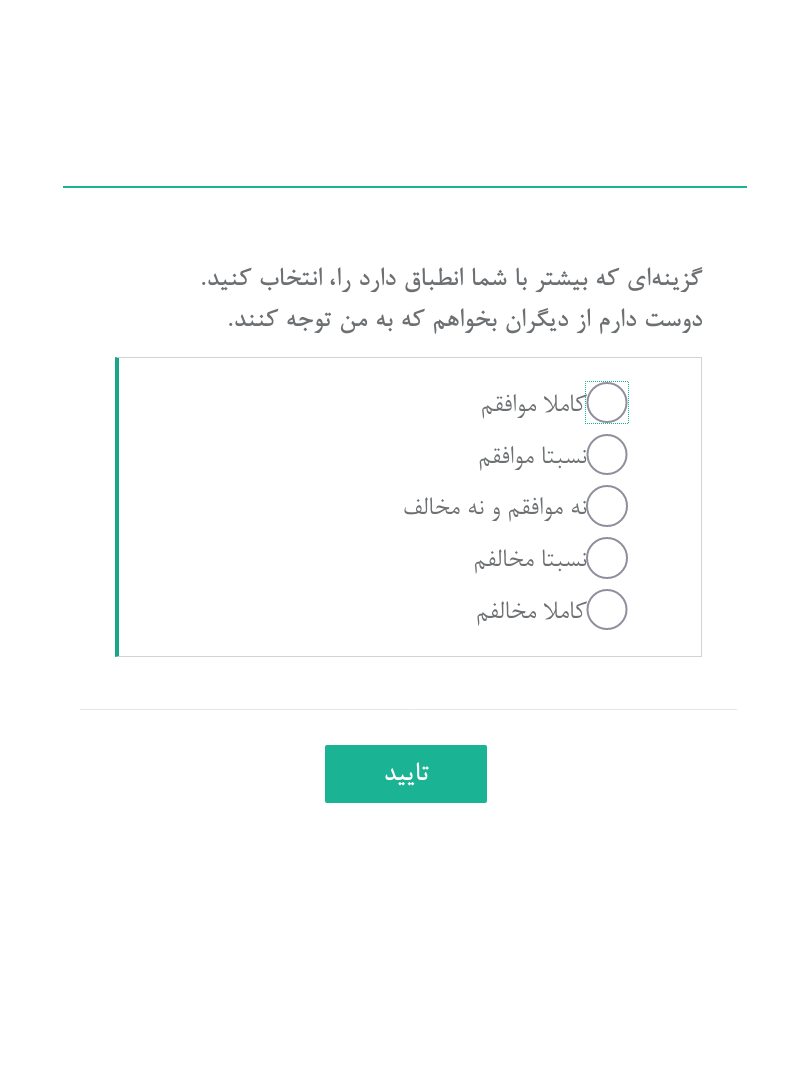
\includegraphics[width=0.8\textwidth,height=0.8\textheight,keepaspectratio]{./img/Task26.png}
\caption{ صفحه 26 آزمایش }
\label{fig:Task26}
\end{figure}
 
 
 % ^ %%%% 
\begin{figure}[htpb]
\centering
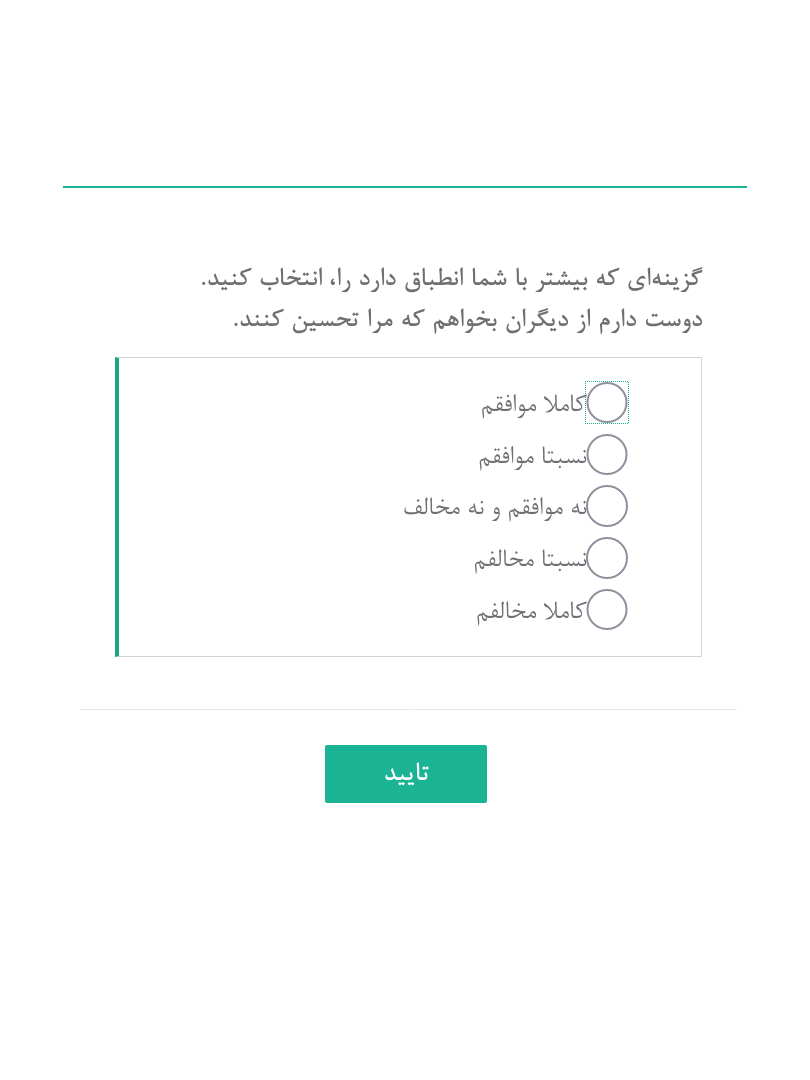
\includegraphics[width=0.8\textwidth,height=0.8\textheight,keepaspectratio]{./img/Task27.png}
\caption{ صفحه 27 آزمایش }
\label{fig:Task27}
\end{figure}
 
 
 % ^ %%%% 
\begin{figure}[htpb]
\centering
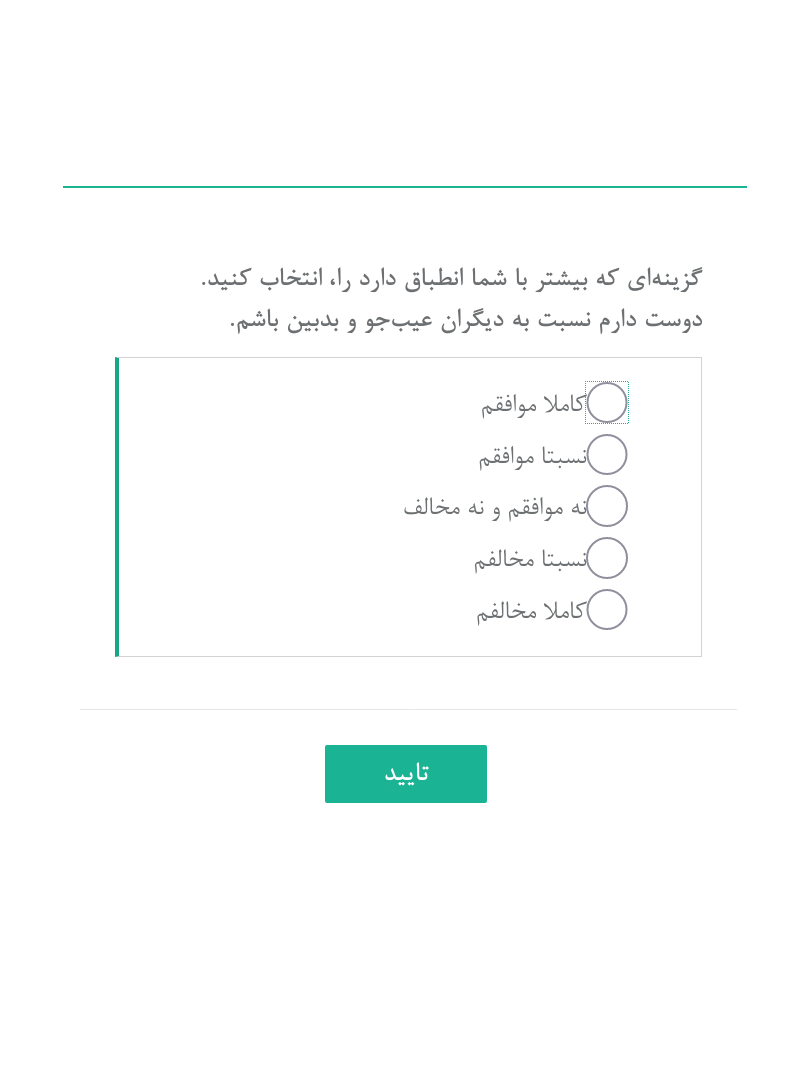
\includegraphics[width=0.8\textwidth,height=0.8\textheight,keepaspectratio]{./img/Task28.png}
\caption{ صفحه 28 آزمایش }
\label{fig:Task28}
\end{figure}
 
 
 % ^ %%%% 
\begin{figure}[htpb]
\centering
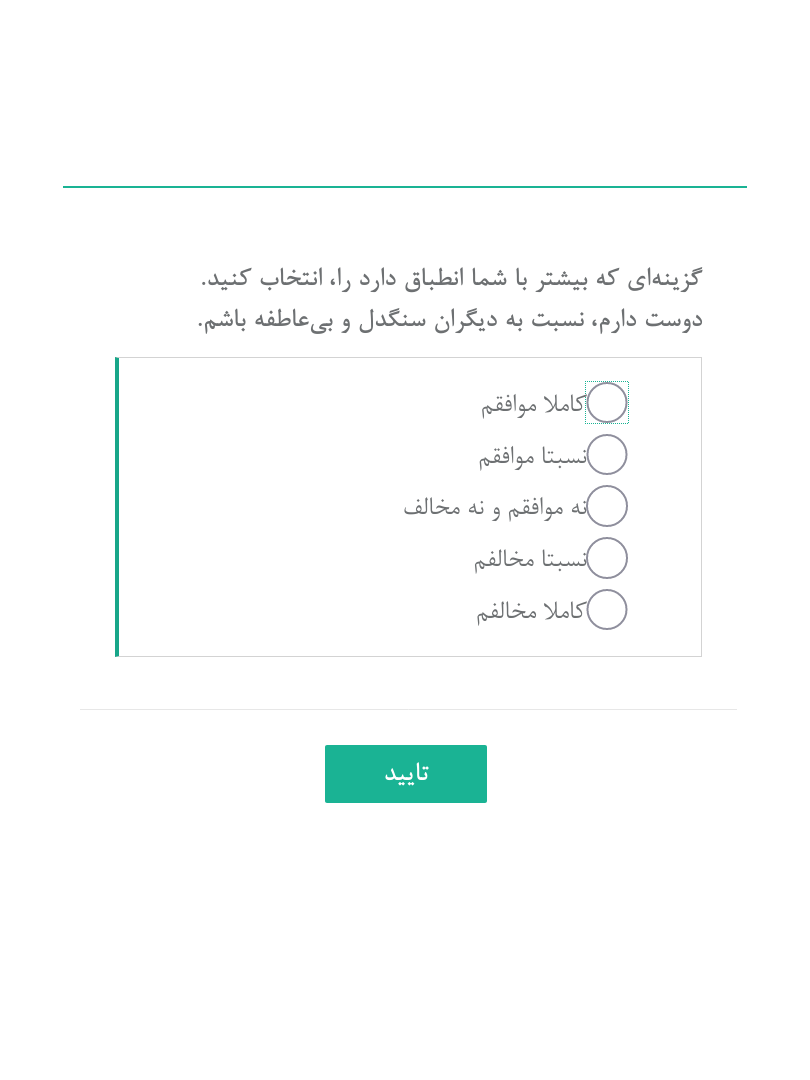
\includegraphics[width=0.8\textwidth,height=0.8\textheight,keepaspectratio]{./img/Task29.png}
\caption{ صفحه 29 آزمایش }
\label{fig:Task29}
\end{figure}
 
 
 % ^ %%%% 
\begin{figure}[htpb]
\centering
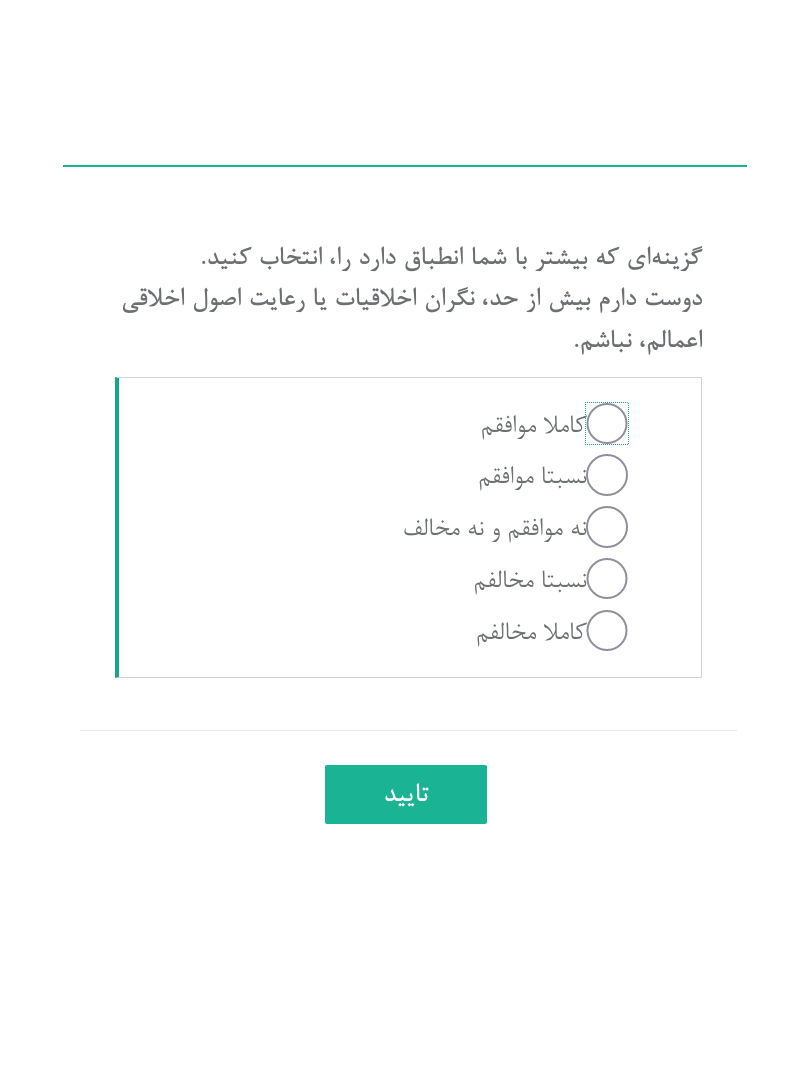
\includegraphics[width=0.8\textwidth,height=0.8\textheight,keepaspectratio]{./img/Task30.png}
\caption{ صفحه 30 آزمایش }
\label{fig:Task30}
\end{figure}
 
 
 % ^ %%%% 
\begin{figure}[htpb]
\centering
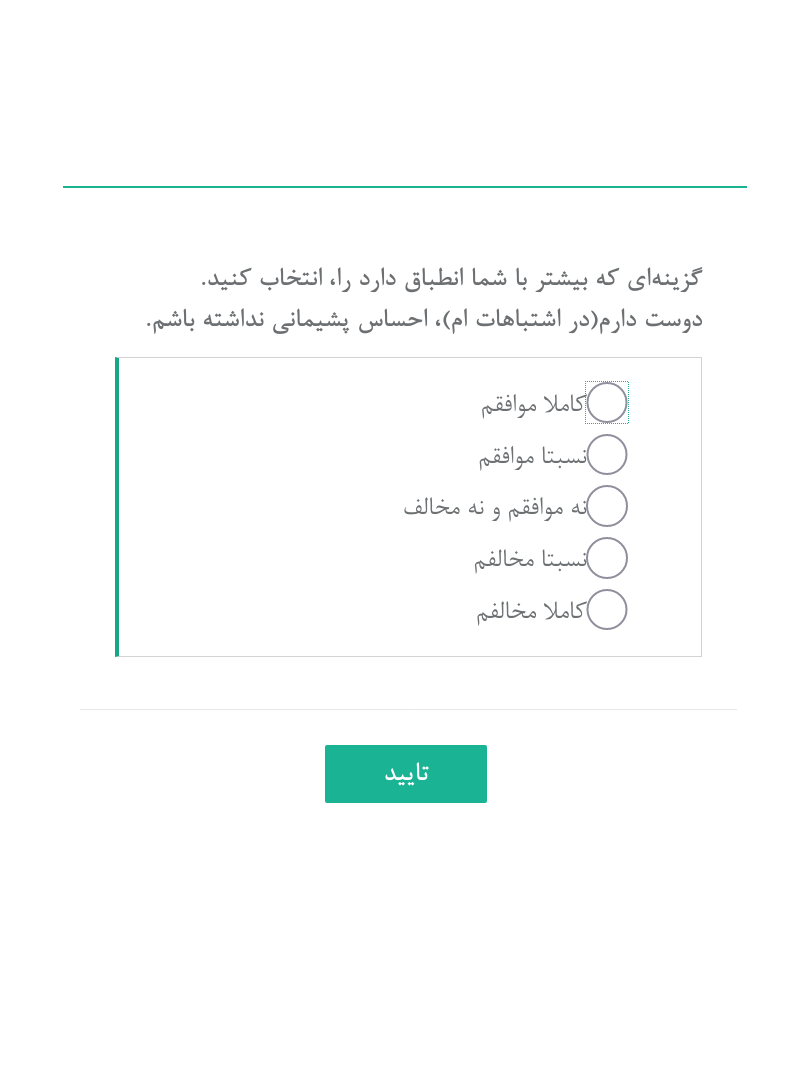
\includegraphics[width=0.8\textwidth,height=0.8\textheight,keepaspectratio]{./img/Task31.png}
\caption{ صفحه 31 آزمایش }
\label{fig:Task31}
\end{figure}
 
 
 % ^ %%%% 
\begin{figure}[htpb]
\centering
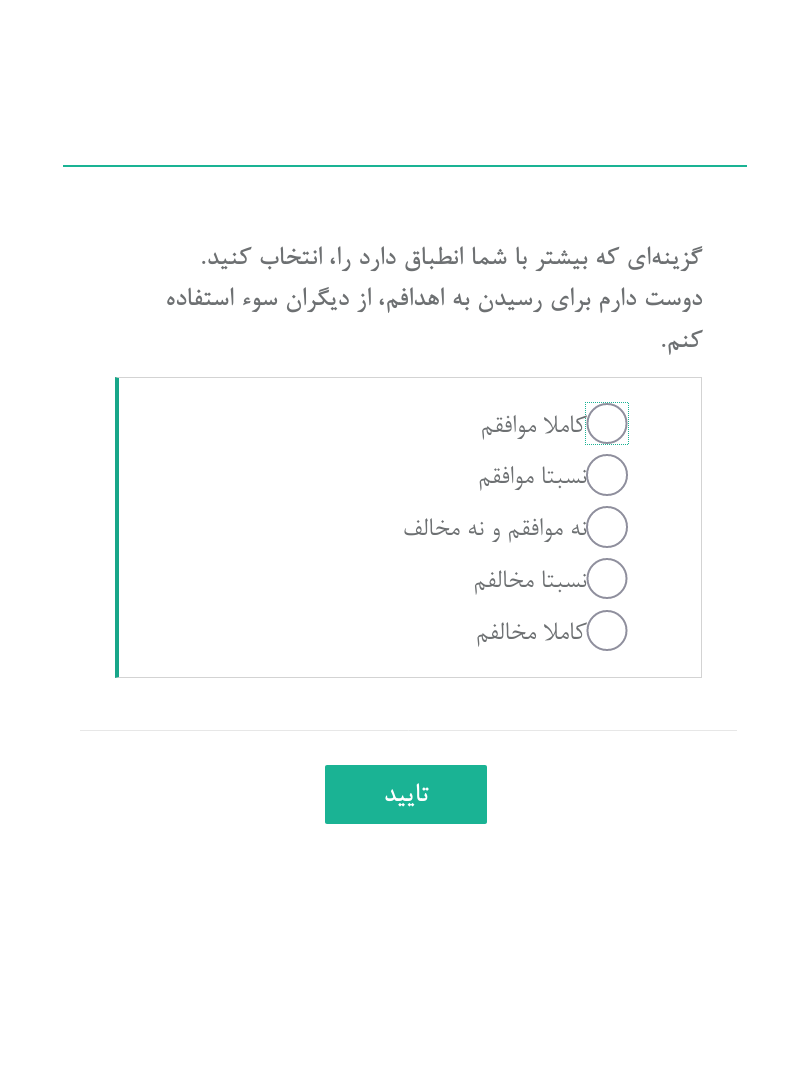
\includegraphics[width=0.8\textwidth,height=0.8\textheight,keepaspectratio]{./img/Task32.png}
\caption{ صفحه 32 آزمایش }
\label{fig:Task32}
\end{figure}
 
 
 % ^ %%%% 
\begin{figure}[htpb]
\centering
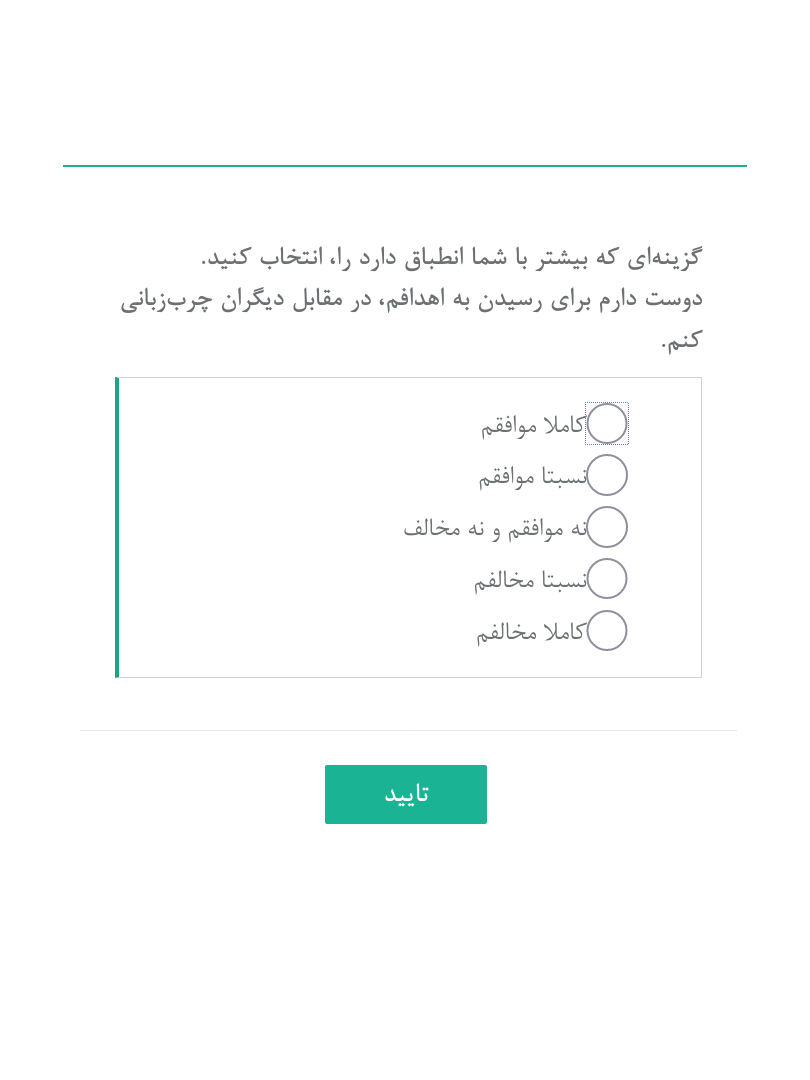
\includegraphics[width=0.8\textwidth,height=0.8\textheight,keepaspectratio]{./img/Task33.png}
\caption{ صفحه 33 آزمایش }
\label{fig:Task33}
\end{figure}
 
 
 % ^ %%%% 
\begin{figure}[htpb]
\centering
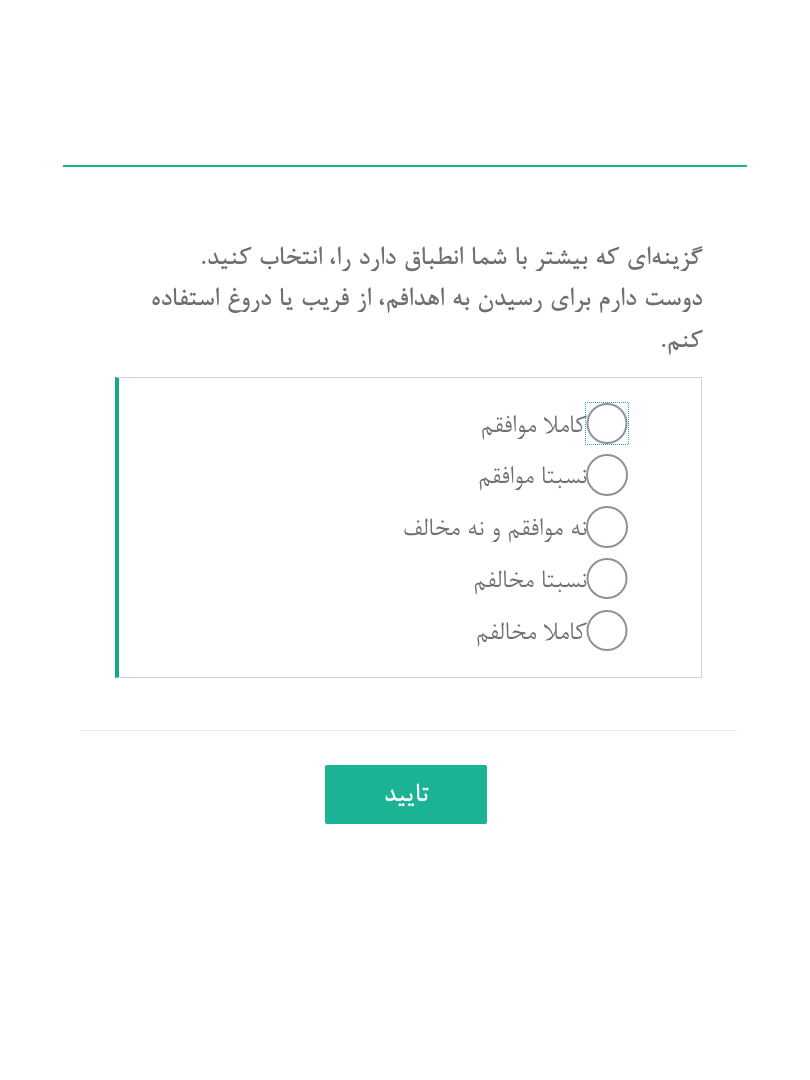
\includegraphics[width=0.8\textwidth,height=0.8\textheight,keepaspectratio]{./img/Task34.png}
\caption{ صفحه 34 آزمایش }
\label{fig:Task34}
\end{figure}
 
 
 % ^ %%%% 
\begin{figure}[htpb]
\centering
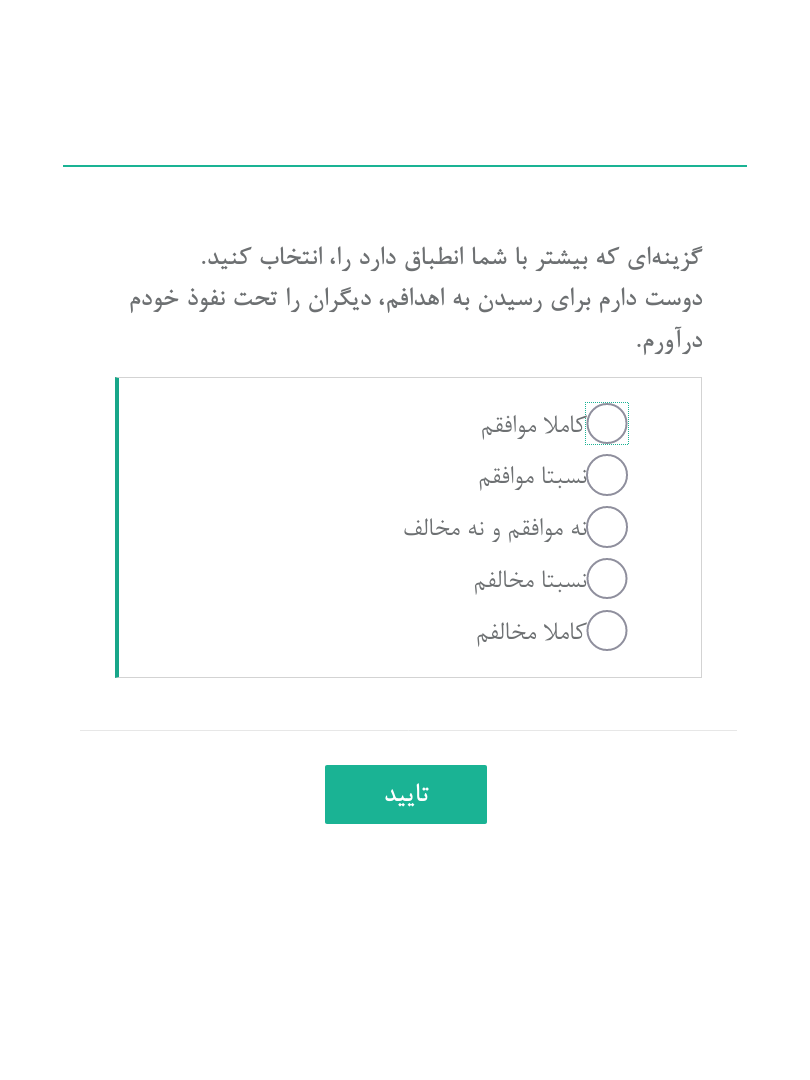
\includegraphics[width=0.8\textwidth,height=0.8\textheight,keepaspectratio]{./img/Task35.png}
\caption{ صفحه 35 آزمایش }
\label{fig:Task35}
\end{figure}
 
 
 % ^ %%%% 
\begin{figure}[htpb]
\centering
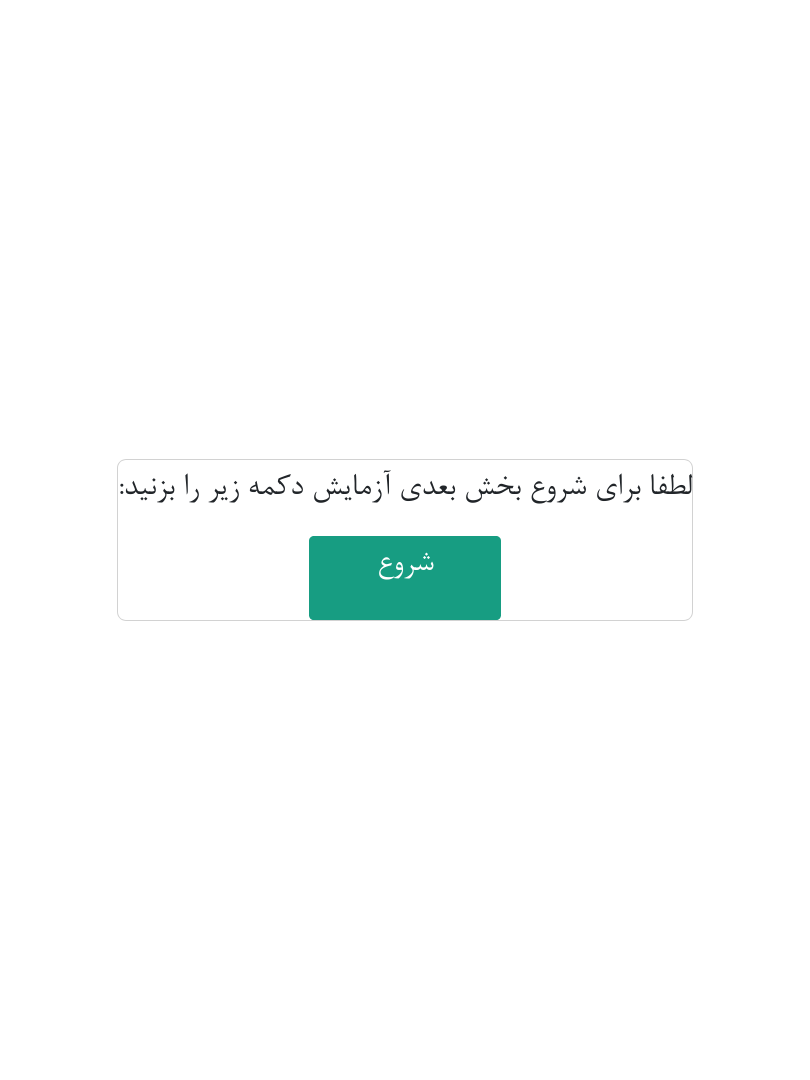
\includegraphics[width=0.8\textwidth,height=0.8\textheight,keepaspectratio]{./img/Task36.png}
\caption{ صفحه 36 آزمایش }
\label{fig:Task36}
\end{figure}
 
 
 % ^ %%%% 
\begin{figure}[htpb]
\centering
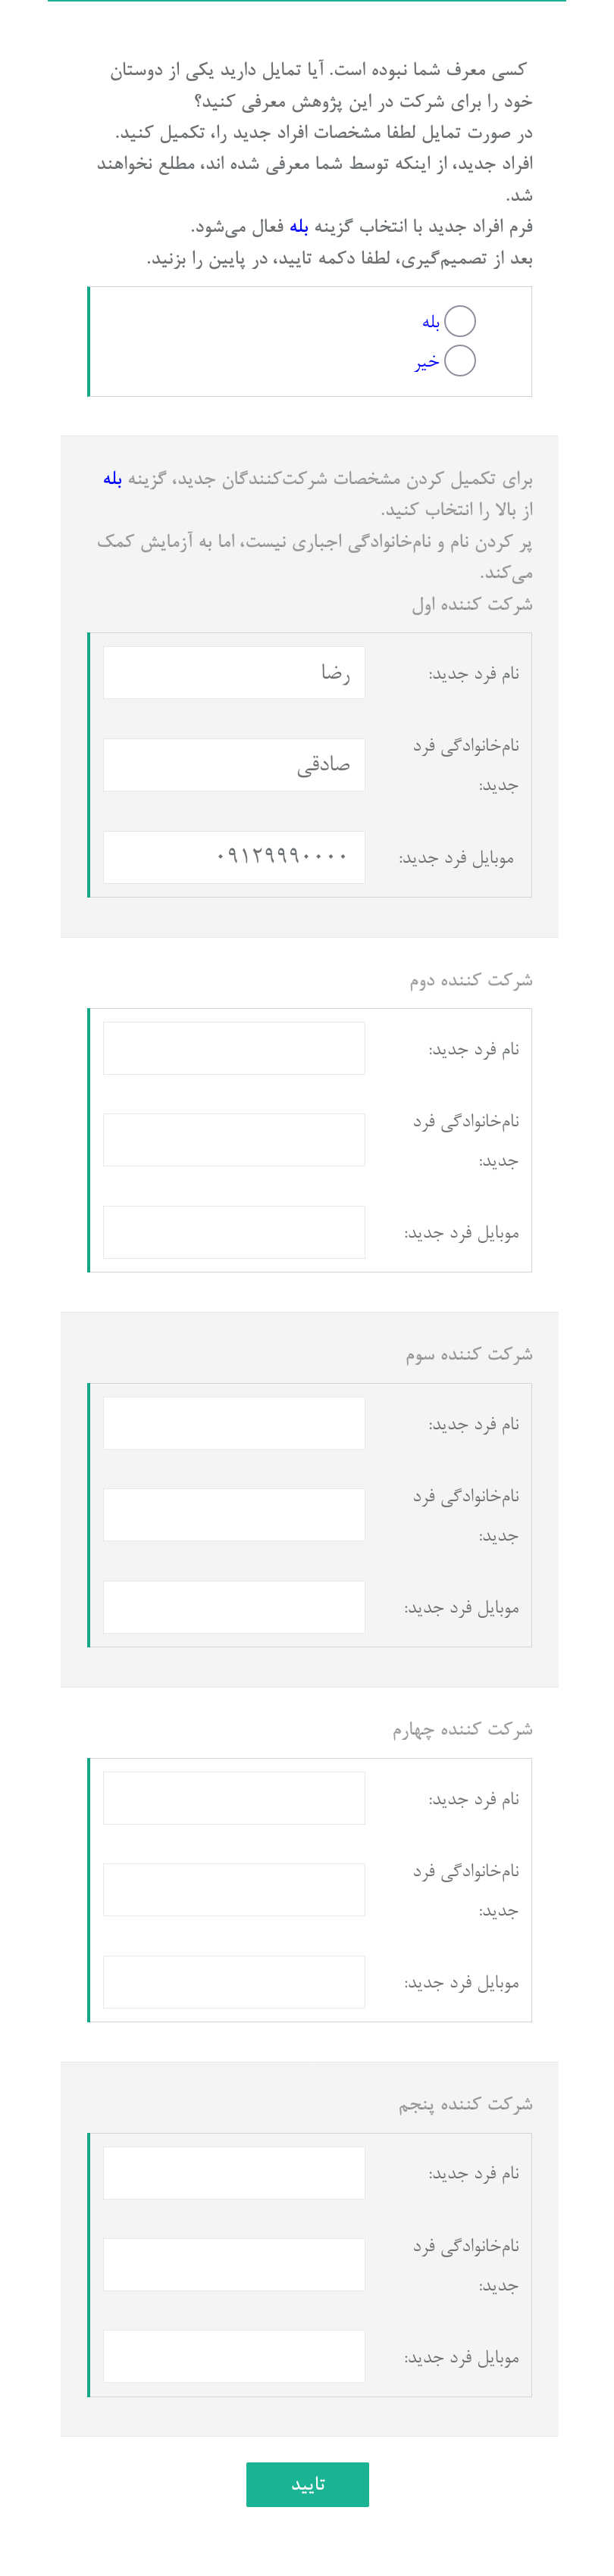
\includegraphics[width=0.8\textwidth,height=0.8\textheight,keepaspectratio]{./img/Task37.png}
\caption{ صفحه 37 آزمایش }
\label{fig:Task37}
\end{figure}
 
 
 % ^ %%%% 
\begin{figure}[htpb]
\centering
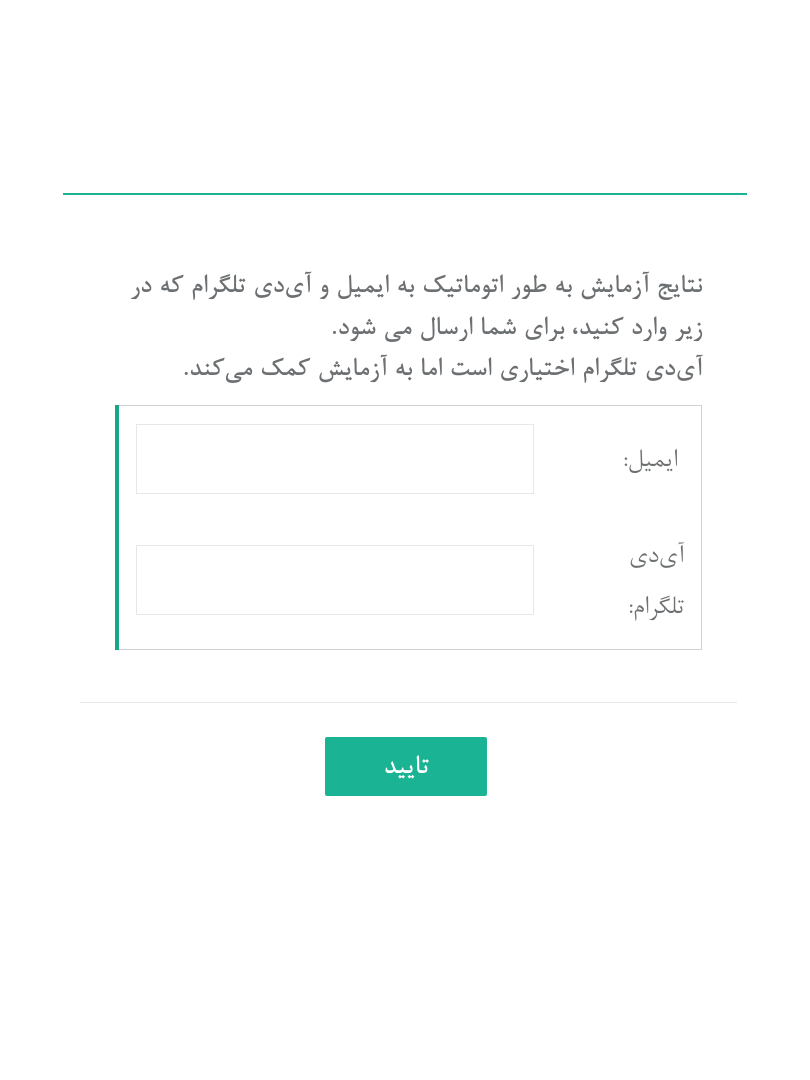
\includegraphics[width=0.8\textwidth,height=0.8\textheight,keepaspectratio]{./img/Task38.png}
\caption{ صفحه 38 آزمایش }
\label{fig:Task38}
\end{figure}
 
 
 % ^ %%%% 
\begin{figure}[htpb]
\centering
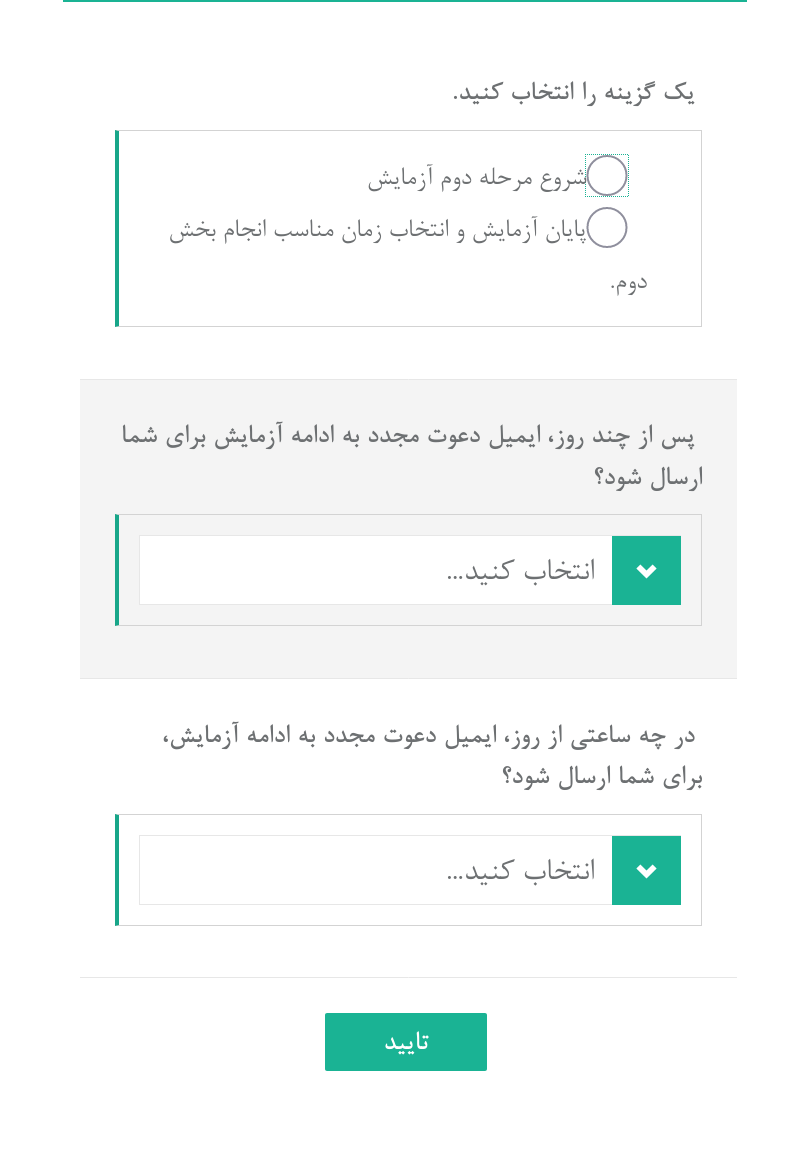
\includegraphics[width=0.8\textwidth,height=0.8\textheight,keepaspectratio]{./img/Task39.png}
\caption{ صفحه 39 آزمایش }
\label{fig:Task39}
\end{figure}
 
 
 % ^ %%%% 
\begin{figure}[htpb]
\centering
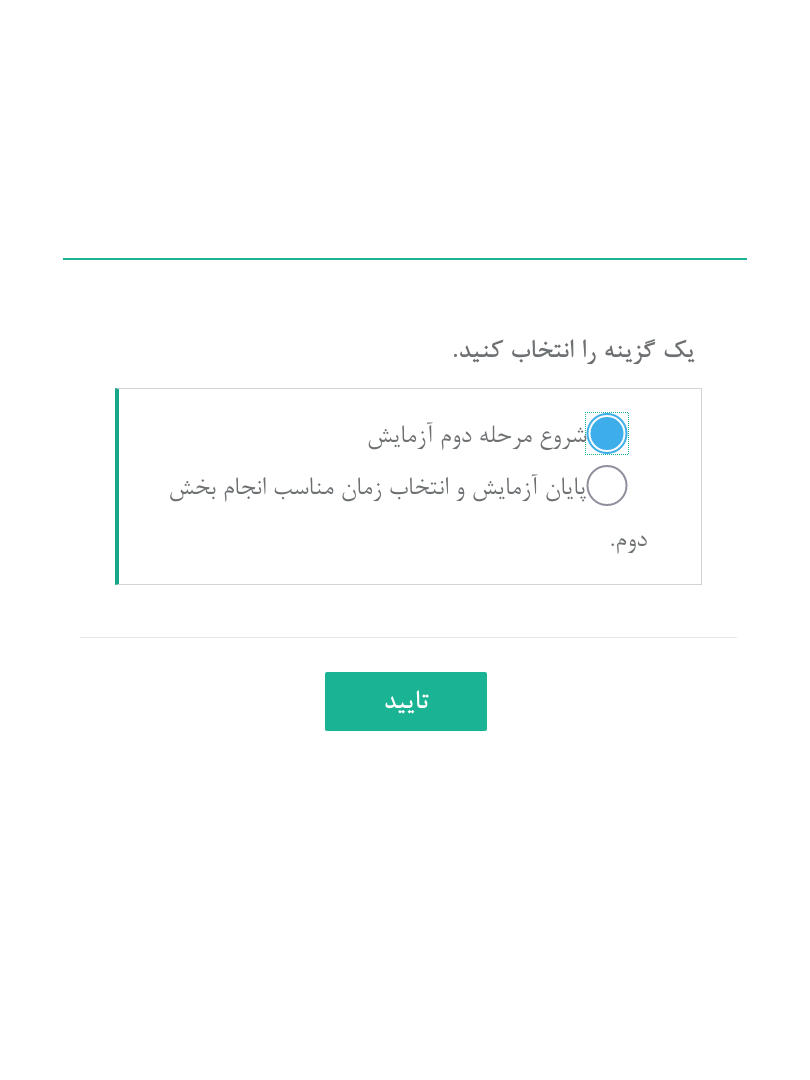
\includegraphics[width=0.8\textwidth,height=0.8\textheight,keepaspectratio]{./img/Task40.png}
\caption{ صفحه 40 آزمایش }
\label{fig:Task40}
\end{figure}
 
 
 % ^ %%%% 
\begin{figure}[htpb]
\centering
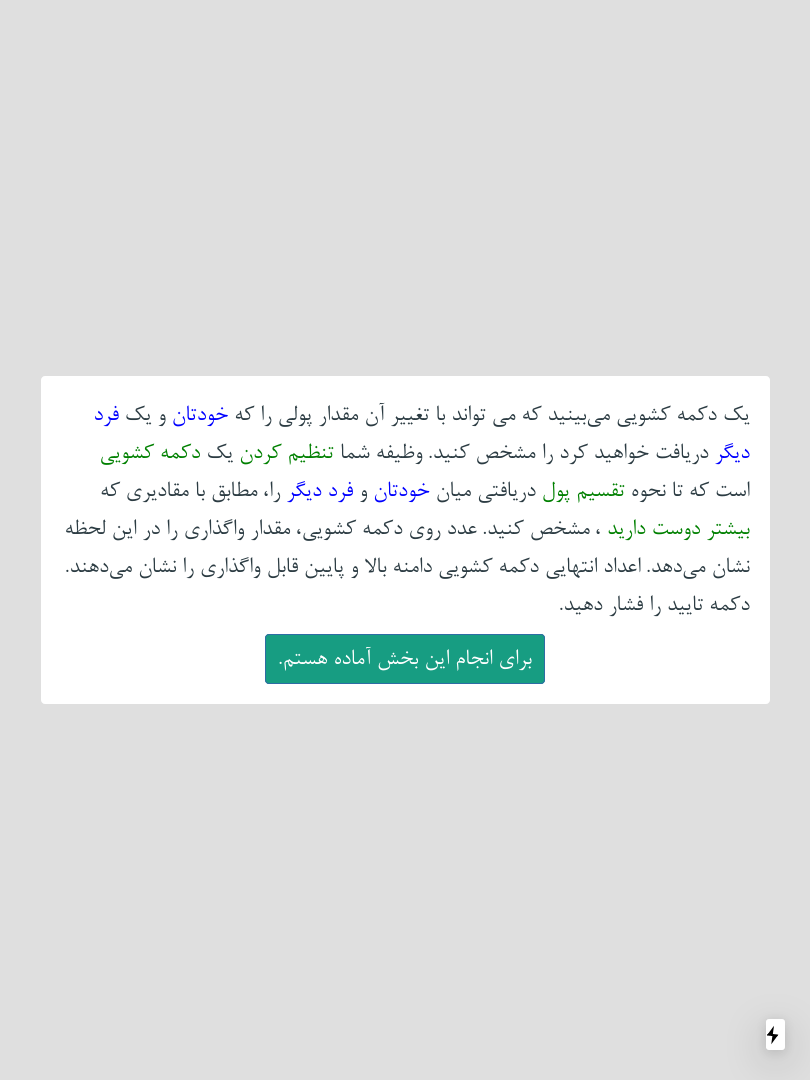
\includegraphics[width=0.8\textwidth,height=0.8\textheight,keepaspectratio]{./img/Task41.png}
\caption{ صفحه 41 آزمایش }
\label{fig:Task41}
\end{figure}
 
 
 % ^ %%%% 
\begin{figure}[htpb]
\centering
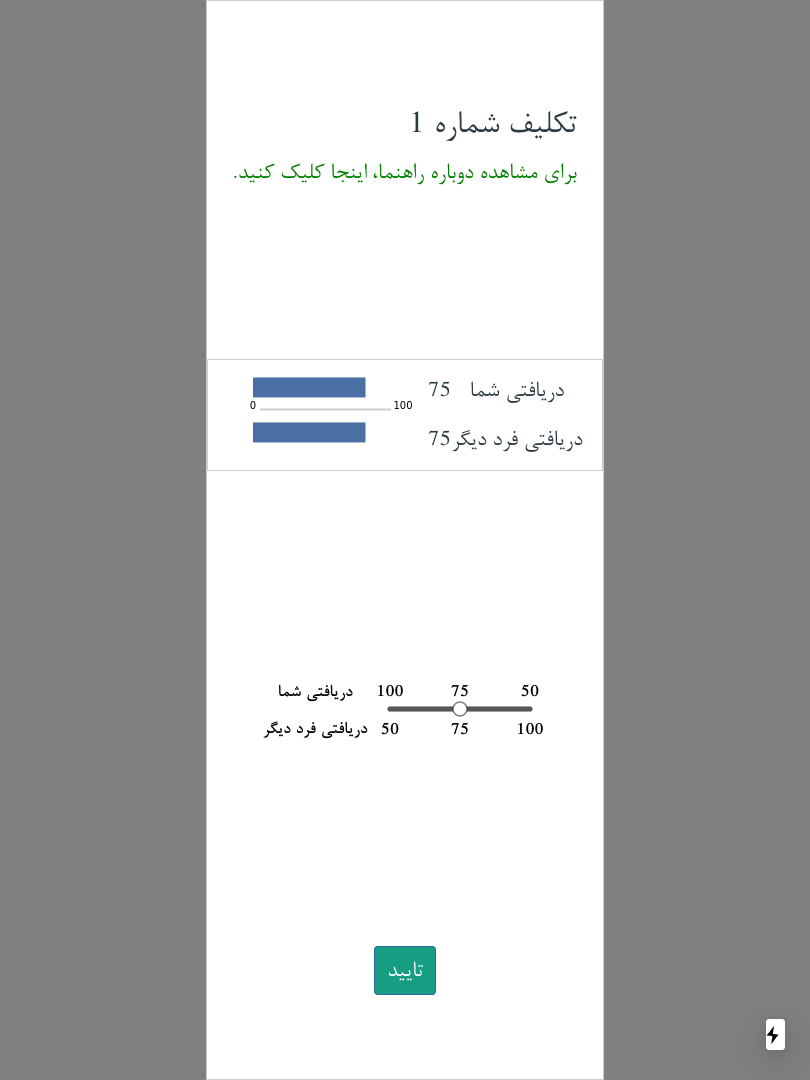
\includegraphics[width=0.8\textwidth,height=0.8\textheight,keepaspectratio]{./img/Task42.png}
\caption{ صفحه 42 آزمایش }
\label{fig:Task42}
\end{figure}
 
 
 % ^ %%%% 
\begin{figure}[htpb]
\centering
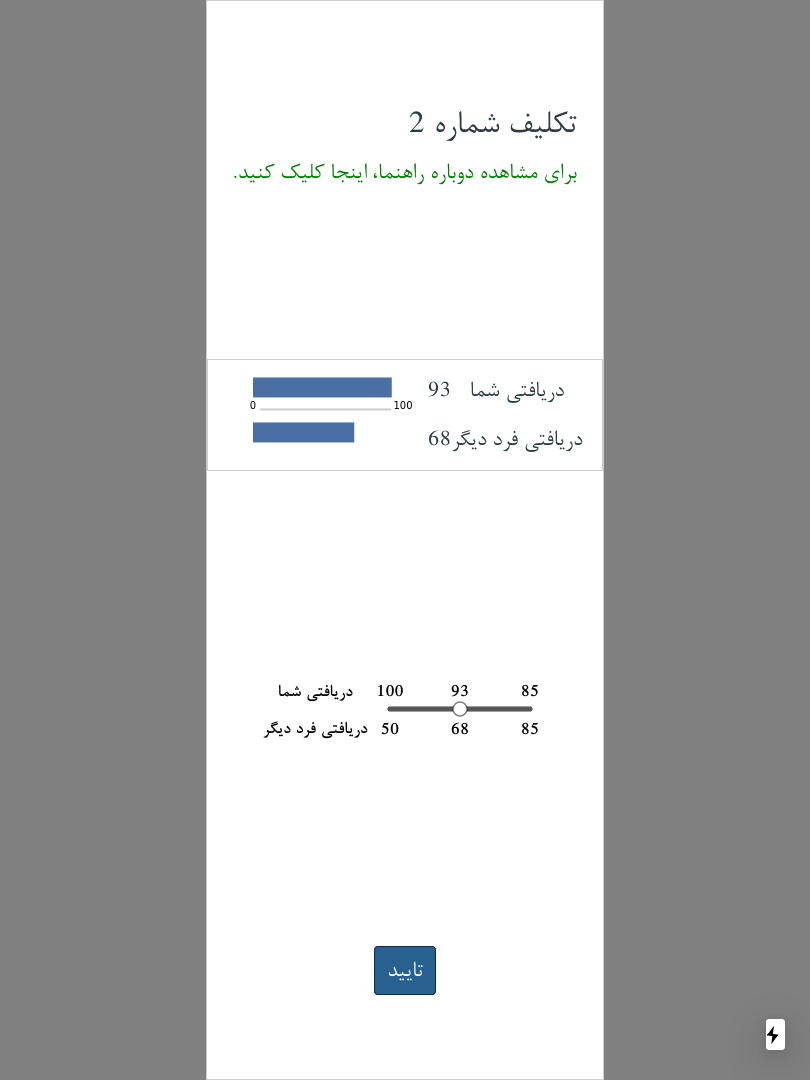
\includegraphics[width=0.8\textwidth,height=0.8\textheight,keepaspectratio]{./img/Task43.png}
\caption{ صفحه 43 آزمایش }
\label{fig:Task43}
\end{figure}
 
 
 % ^ %%%% 
\begin{figure}[htpb]
\centering
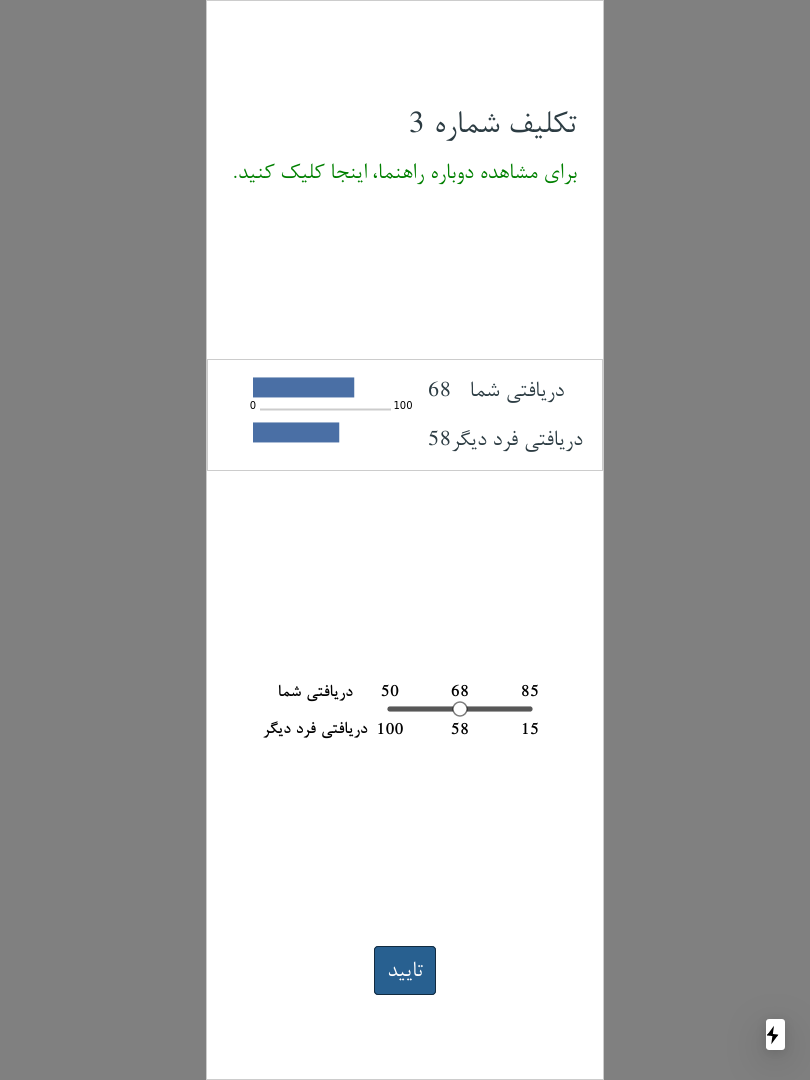
\includegraphics[width=0.8\textwidth,height=0.8\textheight,keepaspectratio]{./img/Task44.png}
\caption{ صفحه 44 آزمایش }
\label{fig:Task44}
\end{figure}
 
 
 % ^ %%%% 
\begin{figure}[htpb]
\centering
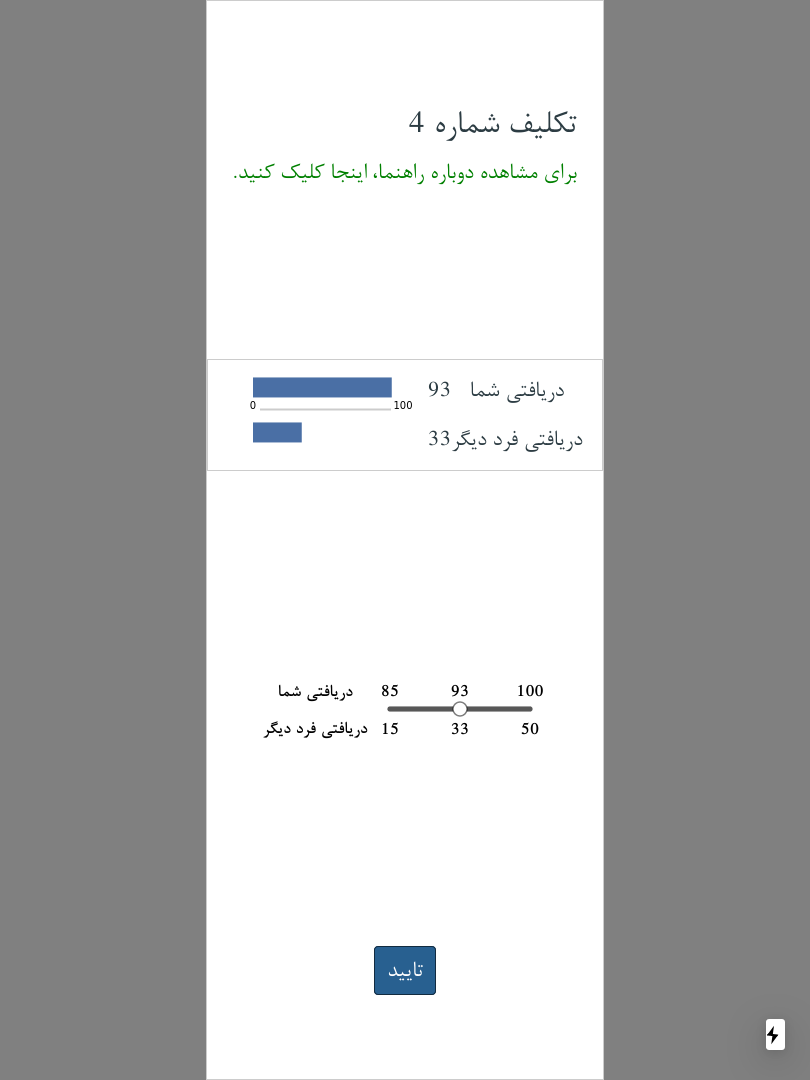
\includegraphics[width=0.8\textwidth,height=0.8\textheight,keepaspectratio]{./img/Task45.png}
\caption{ صفحه 45 آزمایش }
\label{fig:Task45}
\end{figure}
 
 
 % ^ %%%% 
\begin{figure}[htpb]
\centering
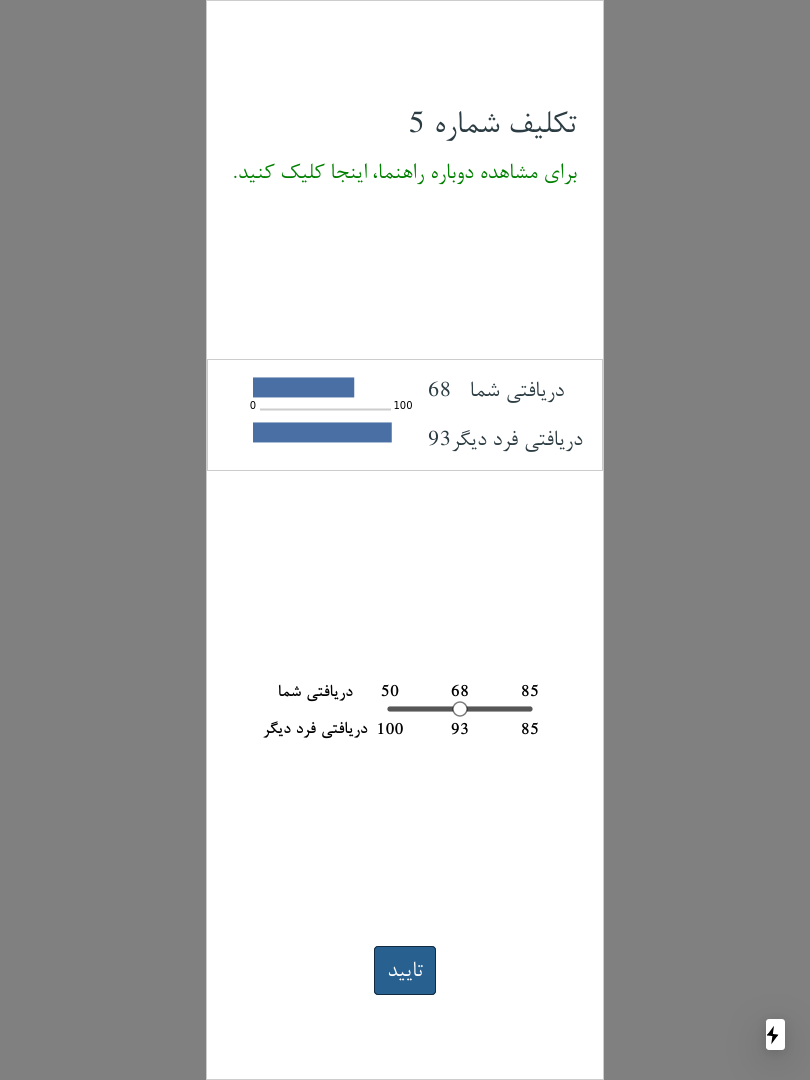
\includegraphics[width=0.8\textwidth,height=0.8\textheight,keepaspectratio]{./img/Task46.png}
\caption{ صفحه 46 آزمایش }
\label{fig:Task46}
\end{figure}
 
 
 % ^ %%%% 
\begin{figure}[htpb]
\centering
\includegraphics[width=0.8\textwidth,height=0.8\textheight,keepaspectratio]{./img/Task47.png}
\caption{ صفحه 47 آزمایش }
\label{fig:Task47}
\end{figure}
 
 
 % ^ %%%% 
\begin{figure}[htpb]
\centering
\includegraphics[width=0.8\textwidth,height=0.8\textheight,keepaspectratio]{./img/Task48.png}
\caption{ صفحه 48 آزمایش }
\label{fig:Task48}
\end{figure}
 
 
%  % ^ %%%% 
% \begin{figure}[htpb]
% \centering
% \includegraphics[width=0.8\textwidth,height=0.8\textheight,keepaspectratio]{./img/Task49.png}
% \caption{ صفحه 49 آزمایش }
% \label{fig:Task49}
% \end{figure}
 
 
%  % ^ %%%% 
% \begin{figure}[htpb]
% \centering
% \includegraphics[width=0.8\textwidth,height=0.8\textheight,keepaspectratio]{./img/Task50.png}
% \caption{ صفحه 50 آزمایش }
% \label{fig:Task50}
% \end{figure}
 
 
%  % ^ %%%% 
% \begin{figure}[htpb]
% \centering
% \includegraphics[width=0.8\textwidth,height=0.8\textheight,keepaspectratio]{./img/Task51.png}
% \caption{ صفحه 51 آزمایش }
% \label{fig:Task51}
% \end{figure}
 
 
%  % ^ %%%% 
% \begin{figure}[htpb]
% \centering
% \includegraphics[width=0.8\textwidth,height=0.8\textheight,keepaspectratio]{./img/Task52.png}
% \caption{ صفحه 52 آزمایش }
% \label{fig:Task52}
% \end{figure}
 
 
%  % ^ %%%% 
% \begin{figure}[htpb]
% \centering
% \includegraphics[width=0.8\textwidth,height=0.8\textheight,keepaspectratio]{./img/Task53.png}
% \caption{ صفحه 53 آزمایش }
% \label{fig:Task53}
% \end{figure}
 
 
%  % ^ %%%% 
% \begin{figure}[htpb]
% \centering
% \includegraphics[width=0.8\textwidth,height=0.8\textheight,keepaspectratio]{./img/Task54.png}
% \caption{ صفحه 54 آزمایش }
% \label{fig:Task54}
% \end{figure}
 
 
%  % ^ %%%% 
% \begin{figure}[htpb]
% \centering
% \includegraphics[width=0.8\textwidth,height=0.8\textheight,keepaspectratio]{./img/Task55.png}
% \caption{ صفحه 55 آزمایش }
% \label{fig:Task55}
% \end{figure}
 
 
%  % ^ %%%% 
% \begin{figure}[htpb]
% \centering
% \includegraphics[width=0.8\textwidth,height=0.8\textheight,keepaspectratio]{./img/Task56.png}
% \caption{ صفحه 56 آزمایش }
% \label{fig:Task56}
% \end{figure}
 
 
%  % ^ %%%% 
% \begin{figure}[htpb]
% \centering
% \includegraphics[width=0.8\textwidth,height=0.8\textheight,keepaspectratio]{./img/Task57.png}
% \caption{ صفحه 57 آزمایش }
% \label{fig:Task57}
% \end{figure}
 
 
%  % ^ %%%% 
% \begin{figure}[htpb]
% \centering
% \includegraphics[width=0.8\textwidth,height=0.8\textheight,keepaspectratio]{./img/Task58.png}
% \caption{ صفحه 58 آزمایش }
% \label{fig:Task58}
% \end{figure}
 
 
%  % ^ %%%% 
% \begin{figure}[htpb]
% \centering
% \includegraphics[width=0.8\textwidth,height=0.8\textheight,keepaspectratio]{./img/Task59.png}
% \caption{ صفحه 59 آزمایش }
% \label{fig:Task59}
% \end{figure}
 
 
%  % ^ %%%% 
% \begin{figure}[htpb]
% \centering
% \includegraphics[width=0.8\textwidth,height=0.8\textheight,keepaspectratio]{./img/Task60.png}
% \caption{ صفحه 60 آزمایش }
% \label{fig:Task60}
% \end{figure}
 
 
%  % ^ %%%% 
% \begin{figure}[htpb]
% \centering
% \includegraphics[width=0.8\textwidth,height=0.8\textheight,keepaspectratio]{./img/Task61.png}
% \caption{ صفحه 61 آزمایش }
% \label{fig:Task61}
% \end{figure}
 
 
%  % ^ %%%% 
% \begin{figure}[htpb]
% \centering
% \includegraphics[width=0.8\textwidth,height=0.8\textheight,keepaspectratio]{./img/Task62.png}
% \caption{ صفحه 62 آزمایش }
% \label{fig:Task62}
% \end{figure}
 
 
%  % ^ %%%% 
% \begin{figure}[htpb]
% \centering
% \includegraphics[width=0.8\textwidth,height=0.8\textheight,keepaspectratio]{./img/Task63.png}
% \caption{ صفحه 63 آزمایش }
% \label{fig:Task63}
% \end{figure}
 
 
%  % ^ %%%% 
% \begin{figure}[htpb]
% \centering
% \includegraphics[width=0.8\textwidth,height=0.8\textheight,keepaspectratio]{./img/Task64.png}
% \caption{ صفحه 64 آزمایش }
% \label{fig:Task64}
% \end{figure}
 
 
%  % ^ %%%% 
% \begin{figure}[htpb]
% \centering
% \includegraphics[width=0.8\textwidth,height=0.8\textheight,keepaspectratio]{./img/Task65.png}
% \caption{ صفحه 65 آزمایش }
% \label{fig:Task65}
% \end{figure}
 
 
%  % ^ %%%% 
% \begin{figure}[htpb]
% \centering
% \includegraphics[width=0.8\textwidth,height=0.8\textheight,keepaspectratio]{./img/Task66.png}
% \caption{ صفحه 66 آزمایش }
% \label{fig:Task66}
% \end{figure}
 
 
%  % ^ %%%% 
% \begin{figure}[htpb]
% \centering
% \includegraphics[width=0.8\textwidth,height=0.8\textheight,keepaspectratio]{./img/Task67.png}
% \caption{ صفحه 67 آزمایش }
% \label{fig:Task67}
% \end{figure}
 
 
%  % ^ %%%% 
% \begin{figure}[htpb]
% \centering
% \includegraphics[width=0.8\textwidth,height=0.8\textheight,keepaspectratio]{./img/Task68.png}
% \caption{ صفحه 68 آزمایش }
% \label{fig:Task68}
% \end{figure}
 
 
%  % ^ %%%% 
% \begin{figure}[htpb]
% \centering
% \includegraphics[width=0.8\textwidth,height=0.8\textheight,keepaspectratio]{./img/Task69.png}
% \caption{ صفحه 69 آزمایش }
% \label{fig:Task69}
% \end{figure}
 
 
%  % ^ %%%% 
% \begin{figure}[htpb]
% \centering
% \includegraphics[width=0.8\textwidth,height=0.8\textheight,keepaspectratio]{./img/Task70.png}
% \caption{ صفحه 70 آزمایش }
% \label{fig:Task70}
% \end{figure}
 
 
%  % ^ %%%% 
% \begin{figure}[htpb]
% \centering
% \includegraphics[width=0.8\textwidth,height=0.8\textheight,keepaspectratio]{./img/Task71.png}
% \caption{ صفحه 71 آزمایش }
% \label{fig:Task71}
% \end{figure}
 
 
%  % ^ %%%% 
% \begin{figure}[htpb]
% \centering
% \includegraphics[width=0.8\textwidth,height=0.8\textheight,keepaspectratio]{./img/Task72.png}
% \caption{ صفحه 72 آزمایش }
% \label{fig:Task72}
% \end{figure}
 
 
%  % ^ %%%% 
% \begin{figure}[htpb]
% \centering
% \includegraphics[width=0.8\textwidth,height=0.8\textheight,keepaspectratio]{./img/Task73.png}
% \caption{ صفحه 73 آزمایش }
% \label{fig:Task73}
% \end{figure}
 
 
%  % ^ %%%% 
% \begin{figure}[htpb]
% \centering
% \includegraphics[width=0.8\textwidth,height=0.8\textheight,keepaspectratio]{./img/Task74.png}
% \caption{ صفحه 74 آزمایش }
% \label{fig:Task74}
% \end{figure}
 
 
%  % ^ %%%% 
% \begin{figure}[htpb]
% \centering
% \includegraphics[width=0.8\textwidth,height=0.8\textheight,keepaspectratio]{./img/Task75.png}
% \caption{ صفحه 75 آزمایش }
% \label{fig:Task75}
% \end{figure}
 
 
%  % ^ %%%% 
% \begin{figure}[htpb]
% \centering
% \includegraphics[width=0.8\textwidth,height=0.8\textheight,keepaspectratio]{./img/Task76.png}
% \caption{ صفحه 76 آزمایش }
% \label{fig:Task76}
% \end{figure}
 
 
%  % ^ %%%% 
% \begin{figure}[htpb]
% \centering
% \includegraphics[width=0.8\textwidth,height=0.8\textheight,keepaspectratio]{./img/Task77.png}
% \caption{ صفحه 77 آزمایش }
% \label{fig:Task77}
% \end{figure}


% %\thispagestyle{empty}
% در این فصل ویژگی‌های مهم و پرکاربرد زی‌پرشین و لاتک معرفی می‌شود. برای راهنمایی بیشتر و به‌کاربردن ویژگی‌های پیشرفته‌تر به راهنمای زی‌پرشین و راهنمای لاتک مراجعه کنید. برای آگاهی از دستورات لاتک که این خروجی را تولید کرده‌اند فایل \lr{appendix1.tex} را ملاحظه فرمایید.
% \footnote{بیشتر مطالب این بخش از مثال 
% \lr{xepersian\_example.tex}
% گرفته شده‌اند که توسط آقای امیرمسعود پورموسی آماده شده است.}

% \section{بندها و زیرنویس‌ها}
% هر جایی از نوشتهٔ خود، اگر می‌خواهید به سر سطر بروید و یک بند (پاراگراف) تازه را آغاز کنید، باید یک خط را خالی بگذارید%
% \footnote{یعنی دوبار باید کلید \lr{Enter} را بزنید.}
%  مانند این:

% حالا که یک بند تازه آغاز شده است، یک زیرنویس انگلیسی%
% \LTRfootnote{English Footnote!}
%  هم می‌نویسیم!
% \section{فرمول‌های ریاضی}
% \label{formula}

% اینجا هم یک فرمول می‌آوریم که شماره دارد:
% \begin{equation}\label{eq:yek}
% A=\frac{c}{d}+\frac{q^2}{\sin(\omega t)+\Omega_{12}}
% \end{equation}
% در لاتک می‌توان به کمک فرمان 
% \lr{\textbackslash label\{\}}
% به هر فرمول یک نام نسبت داد. در فرمول بالا نام \lr{eq:yek} را برایش گذاشته‌ایم (پروندهٔ \lr{tex} همراه با این مثال را ببینید). این نام ما را قادر می‌کند که بعداً بتوانیم با فرمان
% \lr{\textbackslash ref\{eq:yek\}}
% به آن فرمول با شماره ارجاع دهیم. یعنی بنویسیم فرمول \ref{eq:yek}. 
% لاتک خودش شمارهٔ این فرمول‌ها را مدیریت می‌کند.\footnote{یعنی اگر بعداً فرمولی قبل از این فرمول بنویسیم، خودبه‌خود شمارهٔ این فرمول و شمارهٔ ارجاع‌ها به این فرمول یکی زیاد می‌شود. دیگر نگران شماره‌گذاری فرمول‌های خود نباشید!} این هم یک فرمول که شماره ندارد:
% $$A=|\vec{a}\times \vec{b}| + \sum_{n=0}^\infty C_{ij}$$

% این هم عبارتی ریاضی مانند 
% $\sqrt{a^2+b^2}$
%  که بین متن می‌آید.
% \subsection{یک زیربخش}
% \label{zirbakhsh}

% این زیربخش \ref{zirbakhsh} است؛ یعنی یک بخش درون بخش \ref{formula} است.
% \subsubsection{یک زیرزیربخش}
% این هم یک زیرزیربخش است. در لاتک می‌توانید بخش‌های تودرتو در نوشته‌تان تعریف کنید تا ساختار منطقی نوشته را به خوبی نشان دهید. می‌توانید به این بخش‌ها هم با شماره ارجاع دهید، مثلاً بخش فرمول‌های ریاضی شماره‌اش \ref{formula} است.
% \section{نوشته‌های فارسی و انگلیسی مخلوط}
% نوشتن یک کلمهٔ انگلیسی بین متن فارسی بدیهی است، مانند Example در این جمله.
% نوشتن یک عبارت چندکلمه‌ای مانند
%  \lr{More than one word} کمی پیچیده‌تر است.

% اگر ناگهان تصمیم بگیرید که یک بند کاملاً انگلیسی را بنویسید، باید:
% \begin{latin}
% This is an English paragraph from left to right. You can write as much as you want in it.
% \end{latin}
% \section{افزودن تصویر به نوشته}
% پروندهٔ تصویر دلخواه خود را در کنار پروندهٔ \lr{tex} قرار دهید. سپس به روش زیر تصویر را در نوشتهٔ خود بیاورید:
% \begin{latin}
% \begin{verbatim}
% \includegraphics{YourImageFileName}
% \end{verbatim}
% \end{latin}
% به تصویرها هم مانند فرمول‌ها و بخش‌ها می‌توان با شماره ارجاع داد. مثلاً تصویر \ref{fig:shir} یک شیر علاقه‌مند به لاتک را در حال دویدن نشان می‌دهد. برای جزئیات بیشتر دربارهٔ روش گذاشتن تصویرها در نوشته باید راهنماهای لاتک را بخوانید.
% \begin{figure}[ht]
% \centerline{\includegraphics[width=5cm]{lion}}
% \caption{در این تصویر یک شیر علاقه‌مند به لاتک را در حال دویدن می‌بینید.}
% \label{fig:shir}
% \end{figure}

% به تصویرها هم مانند فرمول‌ها و بخش‌ها می‌توان با شماره ارجاع داد. مثلاً تصویر بالا شماره‌اش \ref{fig:shir} است. برای جزئیات بیشتر دربارهٔ روش گذاشتن تصویرها در نوشته باید راهنماهای لاتک را بخوانید.

% \section{محیط‌های شمارش و نکات}
% برای فهرست‌کردن چندمورد، اگر ترتیب برایمان مهم نباشد:
% \begin{itemize}
% \item مورد یکم
% \item مورد دوم
% \item مورد سوم
% \end{itemize}
% و اگر ترتیب برایمان مهم باشد:
    % \begin{enumerate}
    % \item مورد یکم
    % \item مورد دوم
    % \item مورد سوم
    % \end{enumerate}
% می‌توان موردهای تودرتو داشت:
% \begin{enumerate}
% \item مورد ۱
% \item مورد ۲
% \begin{enumerate}
% \item مورد ۱ از ۲
% \item مورد ۲ از ۲
% \item مورد ۳ از ۲
% \end{enumerate}
% \item مورد ۳
% \end{enumerate}
% شماره‌گذاری این موردها را هم لاتک انجام می‌دهد.

% \section{تعریف و قضیه}
% برای ذکر تعریف، قضیه و مثال مثالهای ذیل را ببینید.
% \begin{definition}
% مجموعه همه ارزیابی‌های  (پیوسته)  روی $(X,\tau)$، دامنه توانی احتمالی
% \index{دامنه توانی احتمالی}
% $ X $
% نامیده می‌شود.
% \end{definition}
% \begin{theorem}[باناخ-آلااغلو]
% \index{قضیه باناخ-آلااغلو}
% اگر $ V $ یک همسایگی $ 0 $ در فضای برداری 
% \index{فضای!برداری}
%  توپولوژیکی $ X $ باشد و 
% \begin{equation}\label{eq1}
% K=\left\lbrace \Lambda \in X^{*}:|\Lambda x|\leqslant 1 ; \ \forall x\in V\right\rbrace,
% \end{equation}
% آنگاه $ K $،  ضعیف*-فشرده است که در آن، $ X^{*} $ دوگان
% \index{فضای!دوگان}
%  فضای برداری توپولوژیکی $ X $ است به ‌طوری که عناصر آن،  تابعی‌های 
% خطی پیوسته
% \index{تابعی خطی پیوسته}
%  روی $X$ هستند.
% \end{theorem}
% تساوی \eqref{eq1} یکی از مهم‌ترین تساوی‌ها در آنالیز تابعی است که در ادامه، به وفور از آن استفاده می‌شود.
% \begin{example}
% برای هر فضای مرتب، گردایه 
% $$U:=\left\lbrace U\in O: U=\uparrow U\right\rbrace $$
% از مجموعه‌های بالایی باز، یک توپولوژی تعریف می‌کند که از توپولوژی اصلی، درشت‌تر  است.
% \end{example}
% حال تساوی 
% \begin{equation}\label{eq2}
% \sum_{n=1}^{+\infty} 3^{n}x+7x=\int_{1}^{n}8nx+\exp{(2nx)}
% \end{equation}
% را در نظر بگیرید. با مقایسه تساوی \eqref{eq2} با تساوی \eqref{eq1} می‌توان نتیجه گرفت که ...


% \section{چگونگی نوشتن و ارجاع به مراجع}
% \label{Sec:Ref}


% در لاتک به راحتی می‌توان مراجع خود را نوشت و به آنها ارجاع داد. به عنوان مثال برای معرفی کتاب گنزالس \citep{Gonzalez02book} به عنوان یک مرجع می‌توان آنرا به صورت زیر معرفی نمود:

% \singlespacing
% \begin{LTR}
% \begin{verbatim}
% \bibitem{Gonzalez02book}
% Gonzalez, R.C., and Woods, R.E. {\em Digital Image Processing}, 3rd ed..
% Prentice-Hall, Inc., Upper Saddle River, NJ, USA, 2006.
% \end{verbatim}
% \end{LTR}
% \doublespacing

% در دستورات فوق \lr{Gonzalez02book}  برچسبی است که به این مرجع داده شده است و با استفاده از دستور 
% \verb!\citep{Gonzalez02book}!
% می‌توان به آن ارجاع داد؛ بدون این که شماره‌اش را در فهرست مراجع‌مان بدانیم.

% اگر این اولین مرجع ما باشد در قسمت مراجع به صورت زیر خواهد آمد:\\
% \includegraphics[width=\textwidth]{gonzalez.png}

% این شیوهٔ تعریف مراجع بسیار ابتدایی است و اگر فرمت مراجع، ترتیب یا تعداد آنها را خواسته باشید تغییر دهید، به عنوان مثال ابتدا حرف اول نام نویسنده بیاید و سپس نام خانوادگی، باید همه کارها را به صورت دستی انجام دهید!
% چون در یک \پ یا مقاله باید کنترل کاملی بر مراجع خود داشته باشید و به راحتی بتوانید قالب مراجع را عوض کنید، بنابراین می‌بایست از \lr{Bib\TeX} استفاده کنید که درپیوست  \ref{app:refMan} به  آن پرداخته خواهد شد.
